\documentclass[11pt,a4paper]{article}
\usepackage[margin=2.2cm]{geometry}
\usepackage{amsmath,amssymb}
\usepackage{graphicx}
\usepackage{booktabs}
\usepackage{tabularx}
\usepackage{xcolor}
\usepackage{enumitem}
\usepackage{float}
\usepackage[hidelinks]{hyperref}
\usepackage{caption}
\captionsetup{font=small,labelfont=bf}
\setlist{itemsep=2pt,topsep=3pt}
\graphicspath{{figs/}}
\newcommand{\half}{\tfrac12}
\newcommand{\la}{\ell_a}
\newcommand{\kT}{k_BT}
\newcommand{\keybox}[1]{\par\smallskip\noindent\colorbox{black!6}{\parbox{\dimexpr\linewidth-2\fboxsep}{\small #1}}\par\smallskip}

\title{Overcharged cavities: where the theory stands}
\author{Benjamin Loewe (with Claude)\\[2pt]\small Theory report for Tyler --- 9 October 2026, updated 12 October 2026\\
\small New: escape dynamics (Sec.~\ref{sec:escape}), tilt law across $\lambda$ (Sec.~\ref{sec:tilt}), activity layout (Sec.~\ref{sec:shapes})}
\date{}
\sloppy
\begin{document}
\maketitle

\begin{abstract}
\noindent
An active nematic (NIAMH-MPCD) fills a cavity whose wall anchoring winds $k$ times, so the cavity carries topological charge $k$.
In circles the charge splits into a wall layer of $2k-2$ pinned $+\half$ defects and a bulk of net charge $+1$; a passive cavity instead keeps
all $2k$ $+\half$ at the wall. This report tells the story we now have for why: the anchoring has a $(2k-2)$-fold symmetry, a
wall $+\half$ can sit untilted only on one of its $2k-2$ homeotropic points, and active flow forces the wall defects to a common tilt, which a
ring of $2k$ cannot adopt. Two defects leave, and the remaining ring of $2k-2$ tilts almost for free. Imposing a vortex on a \emph{passive} cavity
reproduces the active structure, so activity enters through the coherent flow it creates; a continuum active nematic (Q-tensor with backflow) organises itself into the same state. Elongating the cavity (aspect ratio $\gtrsim1.3$) destroys
the coherent flow and the layer leaks: wall defects escape 3--7 times faster, independently of one another, and the excess charge circulates as free $+\half$ in
the bulk. The tilt angle itself comes from flow alignment in the no-slip shear at the wall: a flat-wall calculation gives $\tau\simeq\arccos(1/\lambda)=60^\circ$ at leading order for the MPCD nematic, plus a few degrees from the boundary layer and from splay $\neq$ bend, against the measured 61--65$^\circ$ (nearly independent of the order parameter). In active circles the tilt follows $\arccos(1/\lambda)$ within $3^\circ$ for $\lambda=2$--6; below $\lambda\approx2$ the overcharged state itself breaks down. Following single escapes in time, a wall $+\half$ is held mainly by its tilt and by the wall, not by elasticity: the tilt turns its active jet along the wall and the no-slip wall erases the vortex lobe on its wall side, so only $\approx30\%$ of the inward jet acts. An escaper untilts over $\approx40$\,t.u., its missing lobe recovers, the jet straightens inward and the defect runs away, landing on a $\mathcal Q=0$ line like a free $+\half$ (Head et al.). Stronger flow alignment slows exits and refills alike, so these mechanisms set the rates; the steady wall population is a dynamical balance far from the elastic optimum, limited by the crowding of the layer.
\end{abstract}

\keybox{\textbf{The story in seven lines.}
(1) The winding fixes $2k-2$ special wall sites (homeotropic points); tilt and position of a wall $+\half$ are one variable.
(2) Splay $\neq$ bend pins a commensurate ring of $2k-2$ there; a ring of $2k$ is frustrated and unpinned.
(3) Flow tilts the wall defects coherently; the $2k$ ring cannot follow, two defects are ejected: $2k\to2k-2$ at the wall, $+1$ in the bulk.
(4) The bulk active stress drives the flow; the layer acts as an effective planar boundary and brakes it.
(5) In elongated cavities the coherent flow is lost above aspect $\approx1.3$ and the layer leaks defects in proportion to size.
(6) The tilt angle is set by flow alignment in the no-slip shear next to the wall: $\tau\simeq\arccos(1/\lambda)$, confirmed for $\lambda=2$--6.\\
(7) Escape: the tilt and the no-slip wall turn a wall defect's jet along the wall; untilting straightens it inward and the defect runs away. Tilt sets the rates, layer crowding the steady state.}

\tableofcontents
\bigskip

% ======================================================================
\section{System and puzzle}
\paragraph{Simulations.} Two-dimensional nematic MPCD with extensile active dipoles (activity $\zeta=0.07$, active length $\la=22.2\pm0.3$ cells). Walls
impose strong anchoring with lab-frame director angle $\theta=k\phi$ along the wall (arclength-uniform for non-circular walls), so the director winds $k$ times.
Measured Frank constants: splay $K_1\approx42\,\kT$, bend $K_3\approx23\,\kT$. Flow-aligning ($\lambda=2$). Cavities: circles ($R/\la$ = 0.3--2.9,
$k=2$--10, several densities), Cassini ovals and ellipses (aspect 1.1--2.5, $R_\mathrm{eq}=1$--$2\,\la$; 675 runs, 3 seeds).

\paragraph{What we see (Fig.~\ref{fig:maps}).}
\begin{itemize}
  \item \textbf{Passive:} all $2k$ $+\half$ sit in a ring at the wall; nothing in the bulk.
  \item \textbf{Active circle, $R\gtrsim0.8\la$:} $2k-2$ $+\half$ remain pinned at the wall, and the bulk carries net charge $+1$. Free $\pm\half$
        pairs are created and annihilated in the bulk, but the net charge stays $+1$. A single vortex fills the cavity. The wall $+\half$ are tilted by
        $\approx60^\circ$ relative to the normal, with the sign set by the vortex sense.
  \item \textbf{Elongated cavities:} above aspect ratio $\approx1.3$ the single vortex breaks up, the layer loses defects, and the bulk charge grows with size.
\end{itemize}
The question: is the split ``wall $k-1$, bulk $+1$'' topological or geometric, and what mechanism selects it?

\begin{figure}[H]\centering
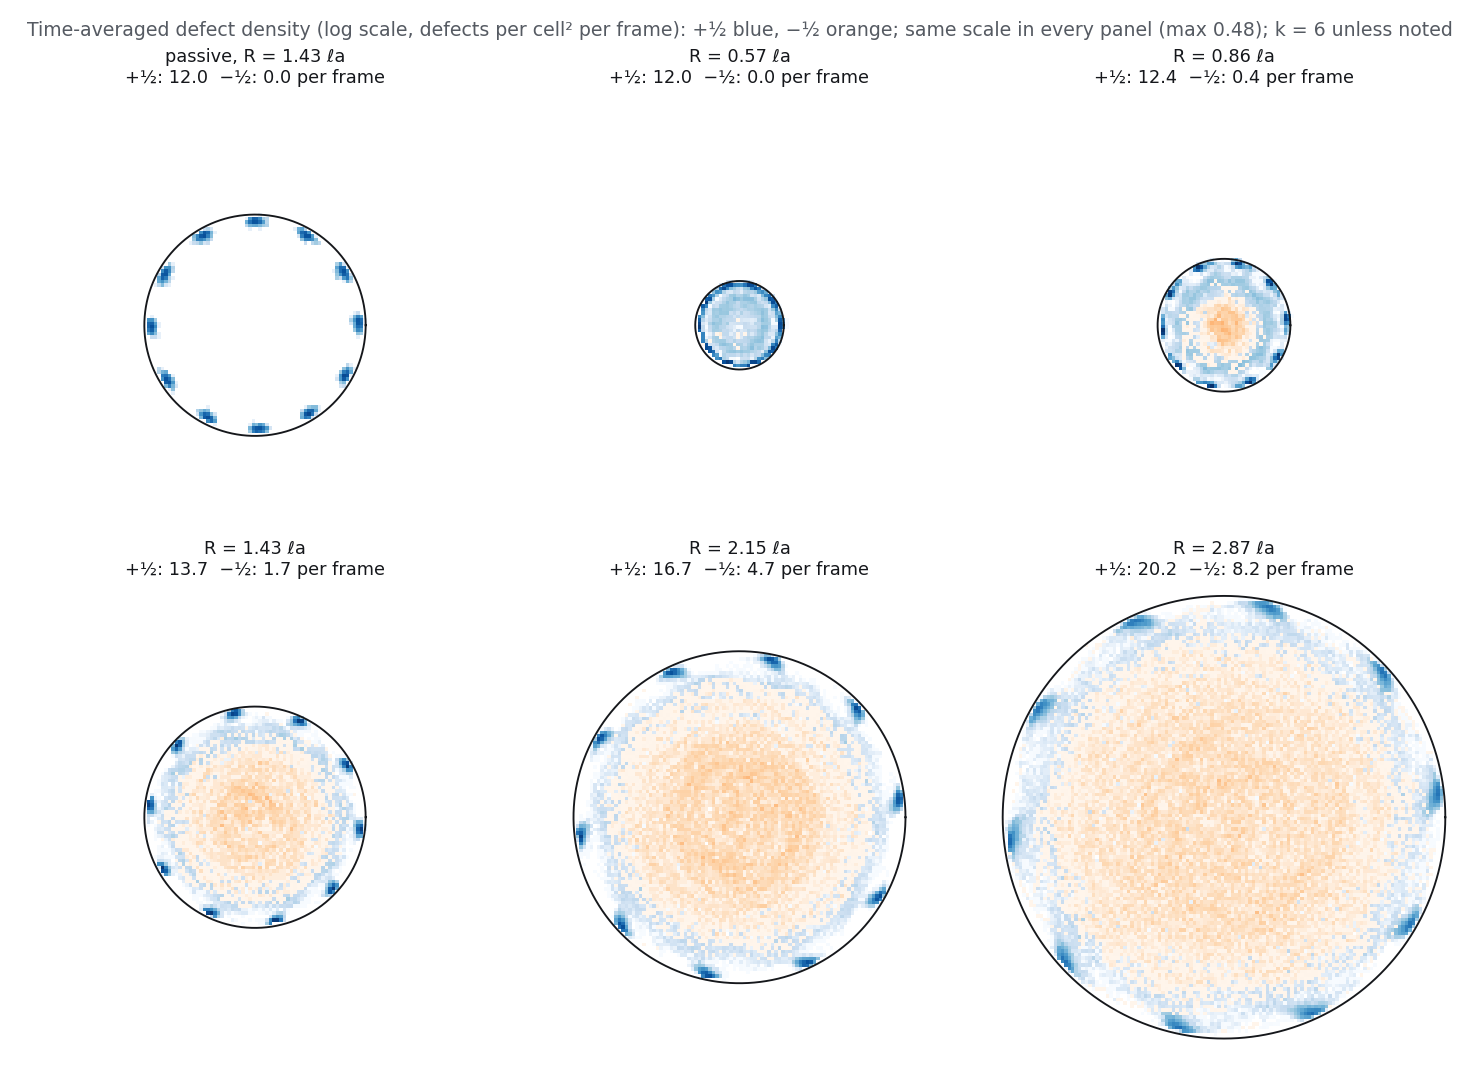
\includegraphics[width=0.85\textwidth]{maps_circles.png}
\caption{Time-averaged defect density in circles, $k=6$ ($+\half$ blue, $-\half$ orange). Top left: passive, 12 $+\half$ at the wall.
Other panels: active, increasing $R/\la$. Above $R\approx0.8\la$ the wall holds 10 sharp sites, and the bulk holds a net $+1$.}\label{fig:maps}
\end{figure}

% ======================================================================
\section{Geometry of the anchoring: $2k-2$ sites and the tilt lock}\label{sec:lock}
\paragraph{Discrete symmetry.} Relative to the local wall normal the anchored director is at angle $(k-1)\phi$: homeotropic where $(k-1)\phi\equiv0$
(mod $\pi$), tangential halfway. Rotating the cavity by $\beta$ changes the pattern unless $(k-1)\beta\equiv0$ (mod $\pi$), so the boundary has a
$(2k-2)$-fold symmetry with homeotropic points at $\phi_n=2\pi n/(2k-2)$ (Fig.~\ref{fig:lock}a). Only $k=1$ is fully rotationally symmetric.

\paragraph{The tilt--position lock.} For a wall $+\half$ at $\phi_j$, its tail angle minus the normal is
\begin{equation}
  \tau_j = 2\psi_\mathrm{rel}(\phi_j) = (2k-2)\phi_j+\text{const}\pmod{2\pi},
\end{equation}
i.e.\ its tail points straight at the wall only at a homeotropic point. The lock holds with concentration 0.99 in $\approx150\,000$ active frames, and locally in
every shape (0.91--0.99, with $\psi_\mathrm{rel}(s)=2\pi k s/P-\phi_n(s)$). Tilt and position are therefore \emph{one} degree of freedom: a common tilt $\tau$ of the whole
ring is a rigid shift of its registry by $\tau/(2k-2)$.

\paragraph{Commensurability.} A ring of $2k-2$ defects can sit untilted with one defect on each homeotropic point (Fig.~\ref{fig:lock}b). A ring of $N$ evenly spaced
defects has consecutive tilts differing by $2(k-1)\cdot2\pi/N$; for $N=2k$ the step is $-2\pi/k$, so the tilts wind twice around the ring and can never all vanish
(Fig.~\ref{fig:lock}c). Measured in passive $k=6$: $+41^\circ,-20^\circ,-91^\circ,\dots$, steps of $-60^\circ$.

\begin{figure}[H]\centering
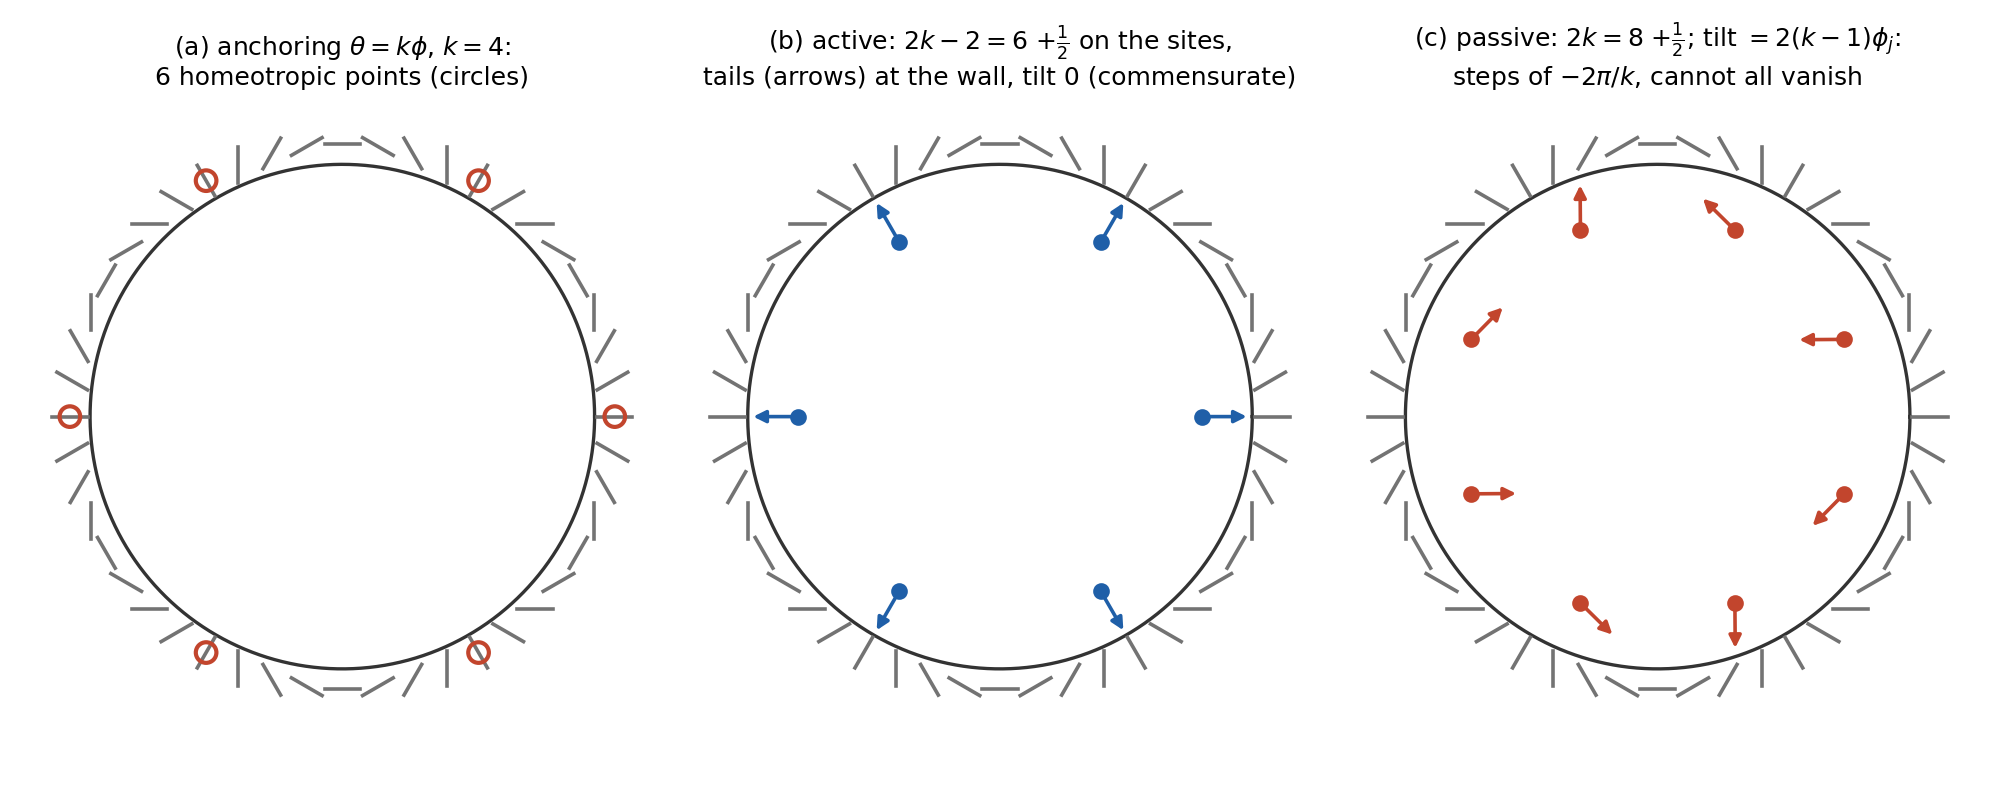
\includegraphics[width=0.95\textwidth]{fig_lock.png}
\caption{Schematic for $k=4$. (a) Anchoring and its $2k-2=6$ homeotropic points. (b) The commensurate ring: one $+\half$ per site, tails (arrows) at the wall,
no tilt. (c) A ring of $2k=8$: by the lock the tilts step by $-2\pi/k$ and wind twice, whatever the registry.}\label{fig:lock}
\end{figure}

\paragraph{Pinning needs splay $\neq$ bend.} With one Frank constant, a uniform rotation of the director costs nothing: rotate the defects by $\beta$, add
$(k-1)\beta$ to the director, and the boundary condition is restored. This gives a free sliding mode. $K_1\neq K_3$ breaks this internal symmetry and turns the
homeotropic points into minima:
\begin{itemize}
  \item \textbf{Active ring ($2k-2$, commensurate):} barrier 80--110\,$\kT$ at $k=6$. Eight runs from six different initial directors all sit at the predicted
        sites (registry $0.03\pm0.07$, resultant 1.00); only the vortex sense is chosen spontaneously. With a sine-modulated winding the active sites follow the
        displaced homeotropic points (0.21--0.27 cells).
  \item \textbf{Passive ring ($2k$, incommensurate):} the lowest harmonics cancel, the barrier is $<1\,\kT$, and the registry is frozen in by the initial condition
        (spontaneous symmetry breaking) and only creeps.
\end{itemize}

\paragraph{Fluctuations.} Along the wall, the harmonic (Hessian) theory of the passive lattice with the measured bend constant reproduces the rms displacement within 2--4\%
with no free parameter. Normal to the wall, a 0.15--0.5 cell excess remains unexplained. Mobility $\mu\approx0.02$.

\paragraph{Half-integer $k$.} For $k\ge2.5$ odd layers (3, 5, 9 wall $+\half$) are pinned on the odd set of homeotropic points with the same lock, tilt and single
vortex. At $k=1.5$ (one site) no layer forms and the flow is weak, as the effective-boundary picture (Sec.~\ref{sec:hydro}) requires at least two sites.

% ======================================================================
\section{Why the active wall holds $2k-2$: flow-induced ejection}\label{sec:ejection}
\paragraph{Mechanism.} A coherent flow aligns the wall defects to a common tilt $\tau$. By the lock, the commensurate $2k-2$ ring adopts this by a registry shift at
almost no cost. The $2k$ ring cannot: its tilts must wind, so forcing a common tilt costs elastic energy. When that frustration exceeds the cost of moving two
$+\half$ into the bulk, two defects are ejected. This leaves the largest ring that can tilt uniformly, and puts a $+1$ in the bulk.

\paragraph{Energetics (Fig.~\ref{fig:energy}).} Frank energy in the anchored disk ($k=6$, $R=31.83$), relaxed outside rigid cores, one-constant and anisotropic:
\begin{itemize}
  \item without flow, ejection costs 155--200\,$\kT$ (the passive state is stable);
  \item forcing a common tilt on the $2k$ ring costs 200--500\,$\kT$ (frustration);
  \item the ejected structure tilts at essentially no cost ($-38$ to $+3\,\kT$); under a common tilt it is cheaper than the forced $2k$ ring by 170--300\,$\kT$.
\end{itemize}

\begin{figure}[H]\centering
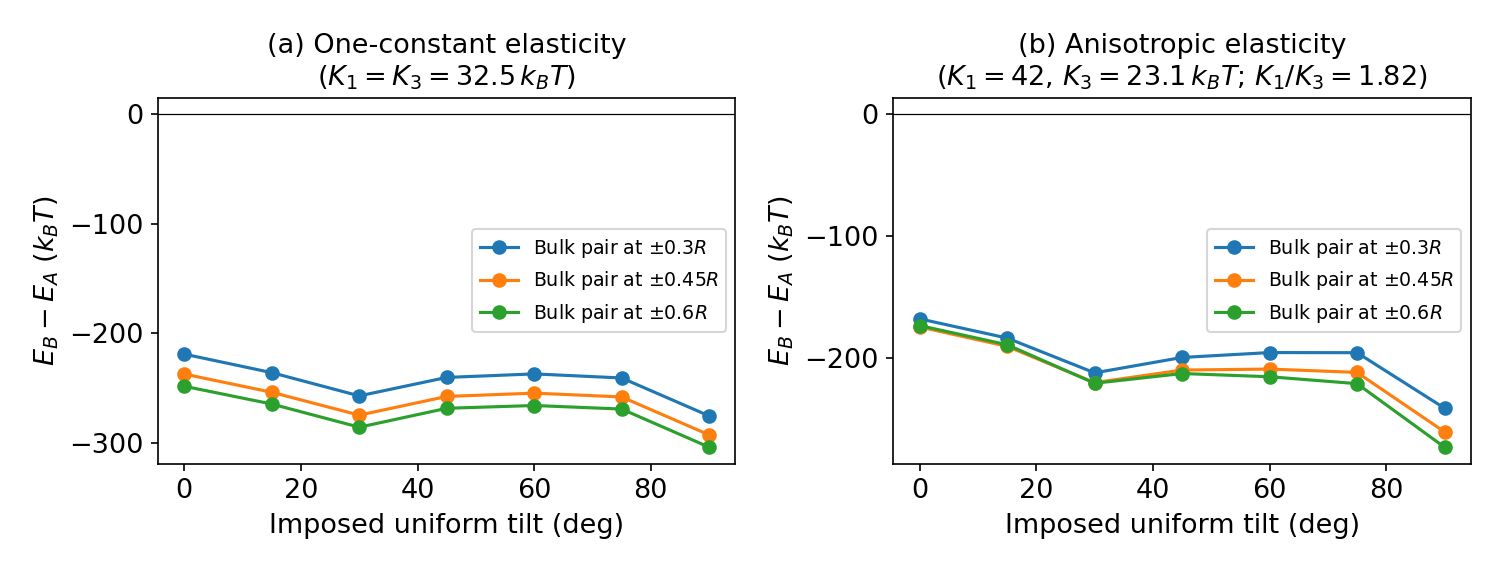
\includegraphics[width=0.85\textwidth]{tilted_structures.png}
\caption{Energy of the ejected structure ($2k-2$ ring plus a bulk pair) minus the $2k$ ring, both with every wall core forced to the same tilt, $k=6$, for three positions
of the bulk pair. (a) one-constant; (b) $K_1=42$, $K_3=23.1$. Negative: ejection favoured. Unforced baseline: $\approx+180\,\kT$.}\label{fig:energy}
\end{figure}

\paragraph{Direct test: passive cavities under an imposed vortex (Fig.~\ref{fig:ejection}).} A solver branch adds an azimuthal body force to a \emph{passive}
cavity, with no activity. Results:
\begin{itemize}
  \item \textbf{Ejection happens:} for $\lambda=2$ and 4 the wall goes $12\to10$ and the bulk acquires $+1$ (0.75--1.0), as in the active state.
  \item \textbf{It needs a common tilt:} with a constant swirl there is no ejection up to $A=0.003$ (tilt coherence 0.2--0.5); at $A=0.01$ both seeds eject, with coherence 0.9--0.96.
  \item \textbf{It needs flow alignment:} partly at $\lambda=1.2$; never for a tumbling nematic ($\lambda=0.5$), which has no aligned angle.
\end{itemize}
Activity therefore enters by \emph{providing the coherent flow}. The tilt angle is set by the layer's response to flow: it grows with $\lambda$ (32$^\circ$ at 0.5,
$\approx60^\circ$ at 1.2--2, 79$^\circ$ at 4). Section~\ref{sec:tilt} shows that this is the flow-aligned angle in the no-slip shear at the wall.

\begin{figure}[H]\centering
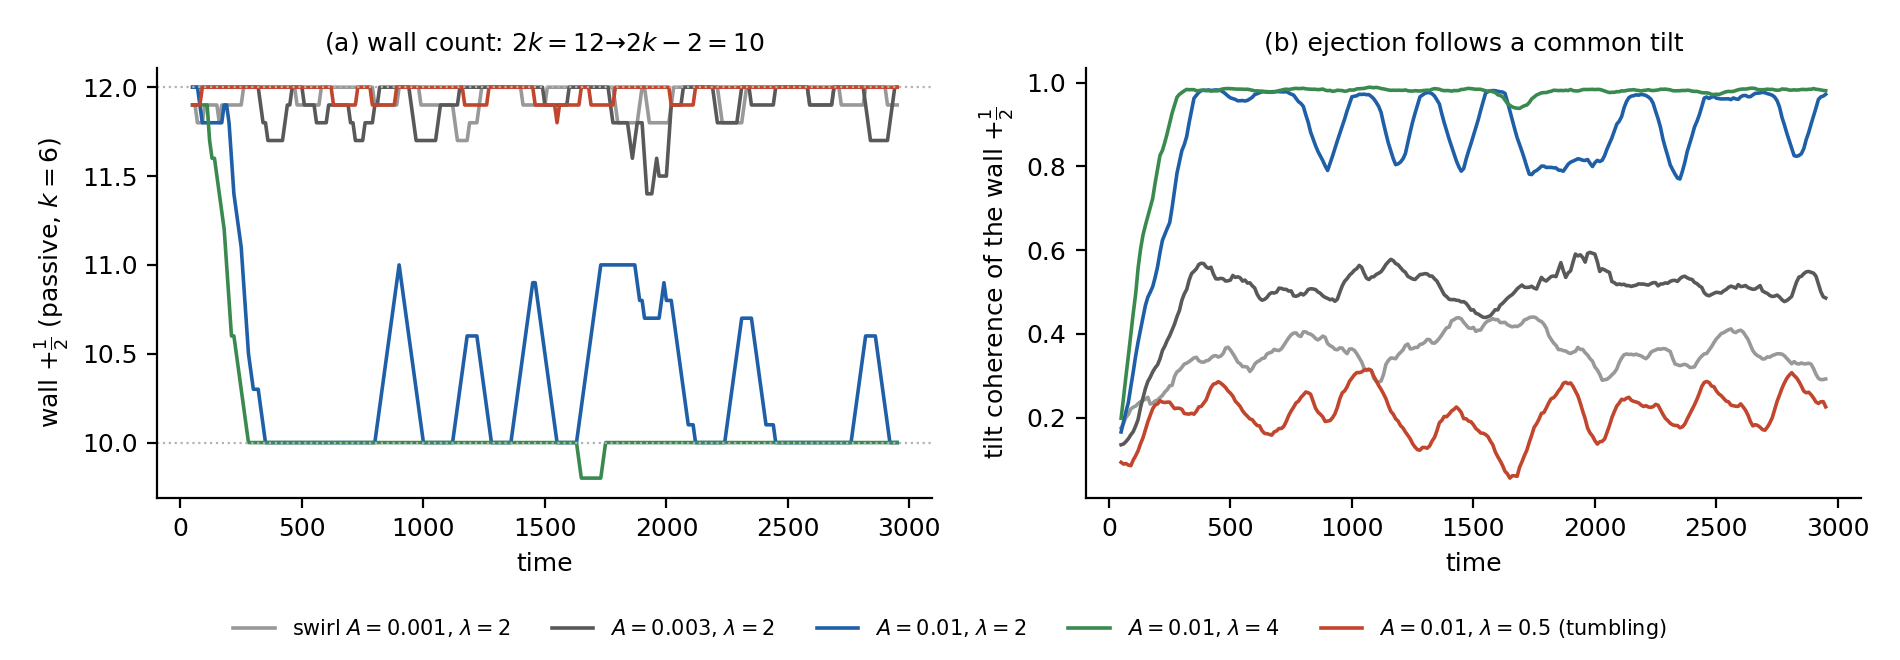
\includegraphics[width=0.95\textwidth]{fig_ejection.png}
\caption{Passive circle, $k=6$, constant imposed swirl $A$ and flow-alignment parameter $\lambda$. (a) Wall $+\half$ count (smoothed). (b) Tilt coherence
$|\langle e^{i\tau_j}\rangle|$ of the wall layer. Ejection to 10 occurs only when the flow is strong enough, and aligning enough, to impose a common tilt.}\label{fig:ejection}
\end{figure}

\paragraph{Mirror prediction ($-k$).} For negative winding the commensurate ring has $2|k-1|$ $-\half$, so the wall should \emph{gain} two $-\half$, with a $+1$ appearing in
the bulk. Energetically favoured by 196--392\,$\kT$ under a common tilt (minus the cost of creating a pair). In passive runs it happens only at $\lambda=4$ (12$\to$13): gaining defects
needs bulk pair creation, rare without activity. This is kinetically blocked, not refuted; a fair test needs activity or a seeded pair.

% ======================================================================
\section{Where the flow comes from: bulk drive, effective boundary}\label{sec:hydro}
\keybox{\textbf{Sign convention.} The angle in \texttt{defects.dat} is the direction of $\nabla\!\cdot Q$, which is the \emph{tail} of a $+\half$. Bulk $+\half$ move against it
(66--72\% of steps, $\approx60\sigma$), as expected for an extensile system. An earlier version of the hydrodynamics used the opposite sign; everything below is corrected.}

\paragraph{The bulk drives, the layer brakes (Fig.~\ref{fig:stokes}).} Stokes flow of the full active force $-\nabla\!\cdot Q$ from the measured director field, with one
positive coefficient, explains 48--72\% of the measured flow. The bulk part alone explains 47--73\%, and it reproduces the two-vortex component in ellipses
(correlation 0.87--0.91). The wall band opposes the circulation: the wall $+\half$ have their tails downstream and their heads pointing into the bulk and upstream.
Point-defect hydrodynamics is not enough: bulk $+\half$ as point forces explain only 6--21\%, and a particle Langevin model (Stokeslets plus log elasticity)
neither keeps $2k-2$ defects at the wall nor makes a circulation.

\begin{figure}[H]\centering
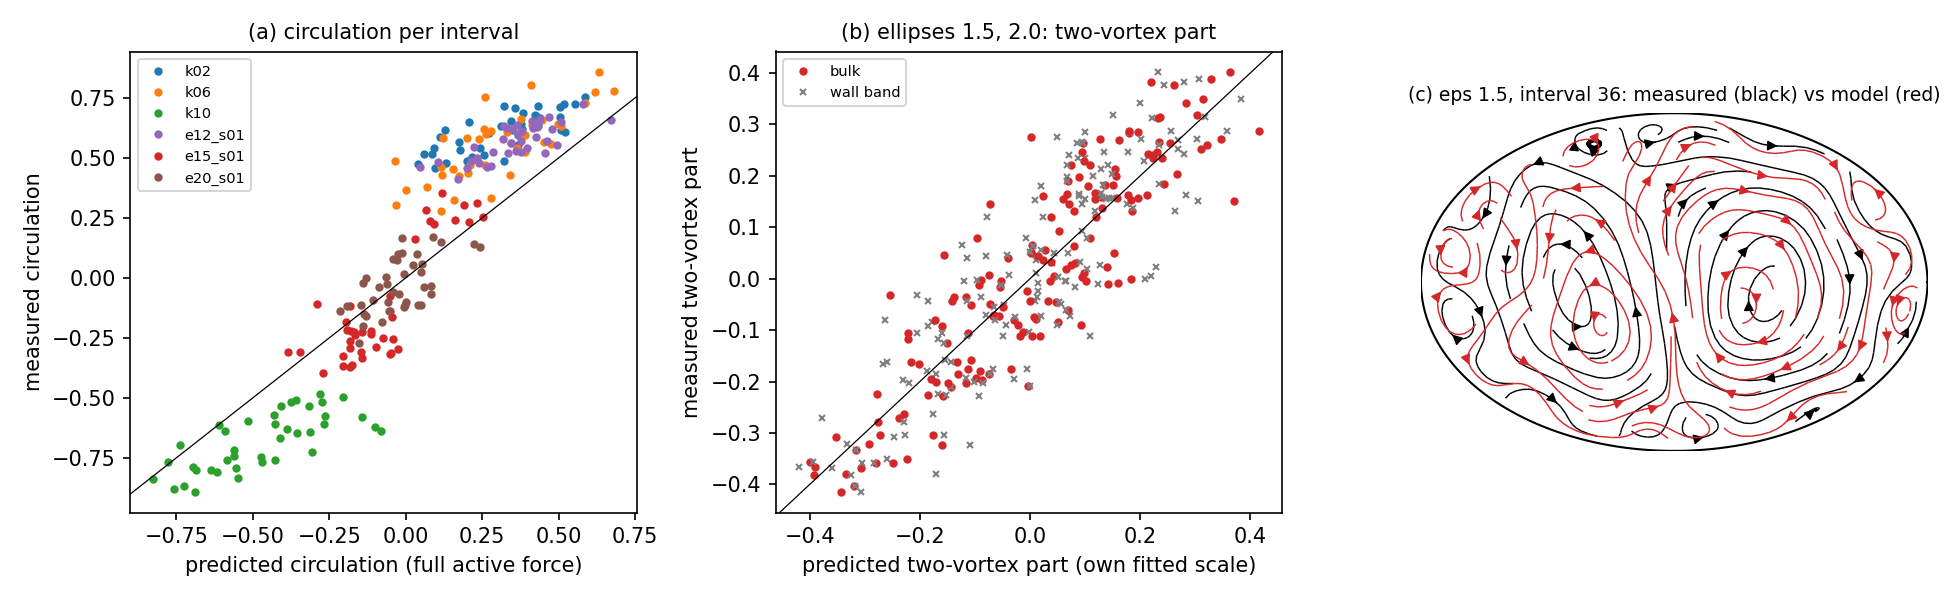
\includegraphics[width=\textwidth]{dirstokes.png}
\caption{Director-field Stokes model. (a) Predicted vs measured circulation per interval (circles $k=2,6,10$; ellipses). (b) Two-vortex component in ellipses
1.5 and 2.0, from the bulk (red) and the wall band (grey). (c) Measured (black) and model (red) streamlines in an ellipse, $\varepsilon=1.5$.}\label{fig:stokes}
\end{figure}

\paragraph{The layer as an effective boundary (Fig.~\ref{fig:effbc}).} Seen from the bulk, the layer of $2k-2$ defects converts the $k$-fold patterned anchoring into an
effectively \emph{planar winding-1} boundary, $\theta=\phi+c$. This is exact in the one-constant limit, and smooth from $\approx0.34$ of the site spacing away from the wall.
A layer tilt $\tau$ turns it into a spiral, $c=90^\circ+\tau/2$, whose extensile stress drives the circulation that tilts the layer. This is a feedback loop through the
elastic field, not through forces at the wall. Its linear stability, with calibrated parameters and one assumed core size, gives the onset of tilt and circulation at
$R/\la\approx0.4$--0.6, where it is measured. The bulk $+1$ is natural in this picture: a winding-1 effective boundary contains net charge $+1$.

\begin{figure}[H]\centering
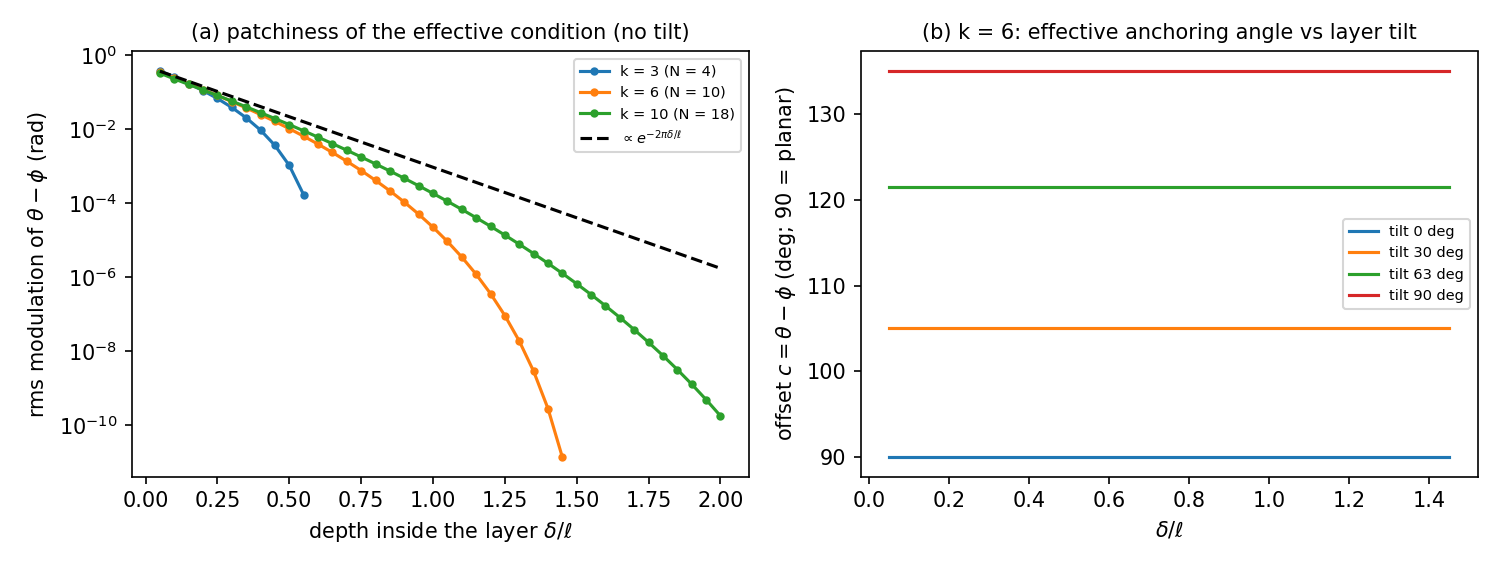
\includegraphics[width=0.8\textwidth]{effective_bc.png}
\caption{(a) The patchiness of the effective condition decays exponentially with depth into the layer. (b) Effective anchoring offset $c$ against the layer tilt: planar
(90$^\circ$) without tilt, a spiral with tilt.}\label{fig:effbc}
\end{figure}

\paragraph{Refinements and what the models still miss.}
\begin{itemize}
  \item Flow alignment rotates the director in the wall layer by about the Leslie angle (measured 26--33$^\circ$ at the defects' depth, Sec.~\ref{sec:tilt}; an earlier estimate of 4--5$^\circ$
        was wrong) and erases the elastic spiral deeper in the active bulk (measured 74--87$^\circ$ vs the elastic 122$^\circ$).
        The azimuthal drive is confined to an annulus $r/R\approx0.6$--0.9 just inside the layer.
  \item Wall defects are not advected (coefficient 0.002--0.004 against fluid speeds 0.13--0.16): the tilted layer sits at a static, shifted registry.
        Under an imposed vortex the active layer is stick--slip: pinned until the flow at its depth reverses, then a jump of the size predicted by the lock.
  \item Size of the tilt: elasticity alone ($K_1\neq K_3$ to second order) locks it at $\approx35^\circ$, not $\approx60^\circ$. The missing ingredient is flow alignment in the no-slip
        shear (Sec.~\ref{sec:tilt}).
  \item The particle model reproduces circulation and tilt once the structure ($2k-2$ at the wall, $+1$ inside) is given, but cannot produce the structure itself.
\end{itemize}

% ======================================================================
\section{The tilt angle: flow alignment in the no-slip shear}\label{sec:tilt}
\paragraph{Question.} Wall $+\half$ tilt by $\approx62^\circ$ in the active circles ($\lambda=2$) and by 57--68$^\circ$ in passive circles under an imposed vortex, growing with the
flow-alignment parameter ($\approx32^\circ$ at $\lambda=0.5$, 57--65$^\circ$ at 1.2, 75--83$^\circ$ at 4) and nearly independent of the flow strength. Elasticity alone gives $\approx35^\circ$.
Does the shear produced by the no-slip wall set the angle?

\paragraph{Continuum test (Fig.~\ref{fig:sheartilt}).} A passive 2D Q-tensor (Beris--Edwards) nematic in the anchored disk ($k=6$, $R=31.83$), one elastic constant, driven by
the measured azimuthal flow of the passive MPCD swirl runs (so the no-slip shear is exactly as in MPCD), no backflow, flow alignment calibrated to $\cos2\theta_L=1/\lambda$ as in MPCD.
Without any fitting it reproduces the MPCD results:
\begin{itemize}
  \item above a flow threshold the 12-ring ejects two defects (wall 10, bulk $+1$); below it the tilt coherence rises gradually (0.07$\to$0.56), then jumps to 1.00 at ejection,
        as in MPCD (0.2--0.5, then 0.9--0.96); $\lambda=1.2$ ejects only at the strongest flow, $\lambda=0.5$ never;
  \item after ejection the tilt is 65--67$^\circ$ at $\lambda=2$ over a $7\times$ range of flow strength, 78--79$^\circ$ at $\lambda=4$, 46$^\circ$ at $\lambda=1.2$; the bulk director sits at the
        Leslie angle $\theta_L$ (29.1/36.7/16.5$^\circ$ vs 30/37.8/16.8$^\circ$).
\end{itemize}
Changing only the flow profile isolates the no-slip shear: shear only in the band next to the wall (rigid bulk) gives the same tilt (67.7 vs 66.7$^\circ$; 79 vs 78$^\circ$);
no shear in that band (rigid rotation there, i.e.\ the wall slips) gives 96--101$^\circ$ and a higher ejection threshold. The angle is set by the shear next to the wall.

\begin{figure}[H]\centering
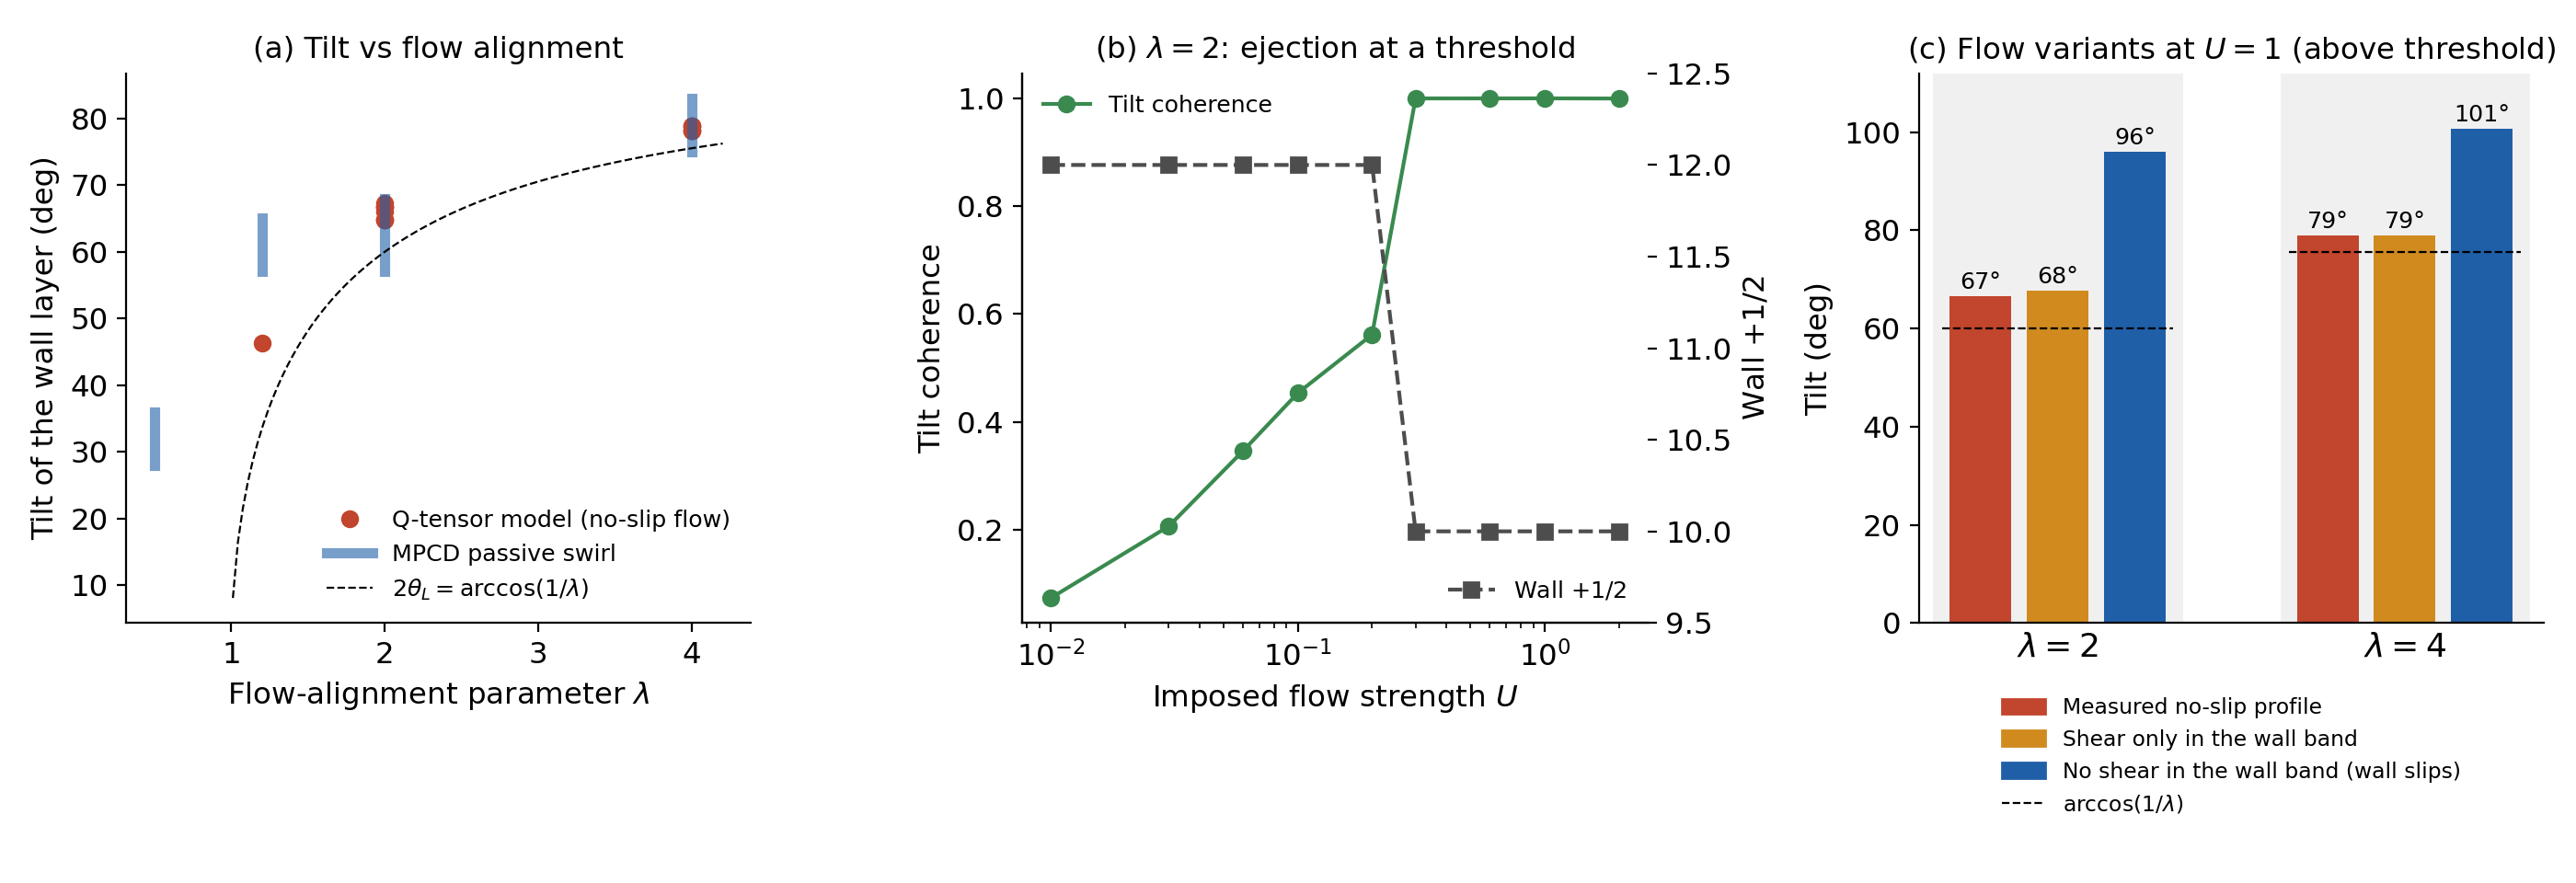
\includegraphics[width=\textwidth]{shear_tilt.png}
\caption{Q-tensor model with the measured no-slip flow. (a) Tilt after ejection vs $\lambda$: model, MPCD passive swirl, $2\theta_L=\arccos(1/\lambda)$. (b) $\lambda=2$: tilt coherence
and wall count vs flow strength. (c) Tilt with the measured profile (red), shear only in the wall band (orange) and no shear in the wall band (blue).}\label{fig:sheartilt}
\end{figure}

\paragraph{With activity instead of an imposed flow.} The same model with Stokes flow, backflow and an extensile active stress (no imposed flow, one elastic constant),
started from the passive ring of 12, organises itself into the active state: at activity $\zeta=0.1$ a single vortex forms (circulation 0.92) but the ring keeps 12 (tilt coherence 0.47);
at $\zeta=0.3$ and 1.0 the vortex ejects two defects (wall 10, bulk $+1$) and the layer tilts coherently by 61.7--62.1$^\circ$ at $\lambda=2$ (MPCD active cavities: $\approx62^\circ$),
independent of the activity; 76.5$^\circ$ at $\lambda=4$, 37.1$^\circ$ at $\lambda=1.2$. The whole chain (activity $\to$ vortex $\to$ ejection $\to$ $2k-2$ wall defects and a bulk $+1$
$\to$ flow-aligned tilt) therefore appears in a continuum active nematic, not only in MPCD.

\paragraph{Flat-wall theory (the local limit; Fig.~\ref{fig:flatwall}).} Wall at $y=0$, simple shear $v_x=sy$ (no slip), periodic along the wall with one site spacing $a_s$;
anchoring $\theta(x,0)=\pi/2+qx$, $q=\pi/a_s$, screened by one $+\half$ per period at depth $d$. Director angle $\theta$ from the wall direction, one-constant Ericksen--Leslie:
\begin{equation}
\gamma_1(\partial_t+\mathbf v\cdot\nabla)\theta = K\nabla^2\theta+\gamma_1\frac{s}{2}\left(\lambda\cos2\theta-1\right).
\end{equation}
\begin{enumerate}
  \item \emph{The layer is a zero mode.} If $\theta_0(x,y)$ is a static solution with the defect at $x=0$, so is $\theta_D=\theta_0(x-D,y)+qD$ (same anchoring, same energy). Sliding the
        defect by $D$ rotates the far field by $\theta_\infty=qD$ and the comet axis by $2qD$: $\tau=2\theta_\infty=2\pi D/a_s$. This is the tilt--position lock of Sec.~\ref{sec:lock}, now derived.
  \item \emph{Leading order.} Beyond the screening length $a_s/2\pi$ the texture is uniform along the wall and the only stable state is the aligned angle $\theta_L$, $\cos2\theta_L=1/\lambda$.
        If the near-wall region passes on no torque, the layer slides along its zero mode until $\theta_\infty=\theta_L$:
        \begin{equation}\tau_0=2\theta_L=\arccos(1/\lambda),\end{equation}
        independent of $s$, $K$ and $\gamma_1$. Only the ratio of strain to vorticity matters, and the no-slip wall fixes it (simple shear).
  \item \emph{Boundary-layer correction.} Linearising about $\theta_L$ gives an alignment length $\ell_E=\sqrt{K/(\gamma_1 s\sqrt{\lambda^2-1})}$; a torque $\Gamma$ per unit length from the
        band between the wall and the defects over-rotates the layer by $\Gamma\ell_E/K$. With the ansatz $\Gamma=\gamma_1 sd/2$ (in the band the anchoring holds the director, so only
        the vorticity acts):
        \begin{equation}\tau=\arccos\frac1\lambda+d\sqrt{\frac{\gamma_1 s}{K}}\,(\lambda^2-1)^{-1/4}.\label{eq:tilt}\end{equation}
\end{enumerate}
Flat-wall Q-tensor simulations confirm all three steps: the far field aligns at $\theta_L$ within $1^\circ$; the registry shift equals the tilt; at weak shear $\tau\to\arccos(1/\lambda)$;
and Eq.~\eqref{eq:tilt} matches 35 runs ($\lambda=1.1$--4, a $100\times$ range of shear, $a_s=10$--40) with no free parameter (ratio 0.97, correlation 0.98). Steps 1--2 and the
form of step 3 are derived; the prefactor $\gamma_1 sd/2$ is an ansatz (a first-principles projection onto the zero mode fails, because it is dominated by the defect core).

\begin{figure}[H]\centering
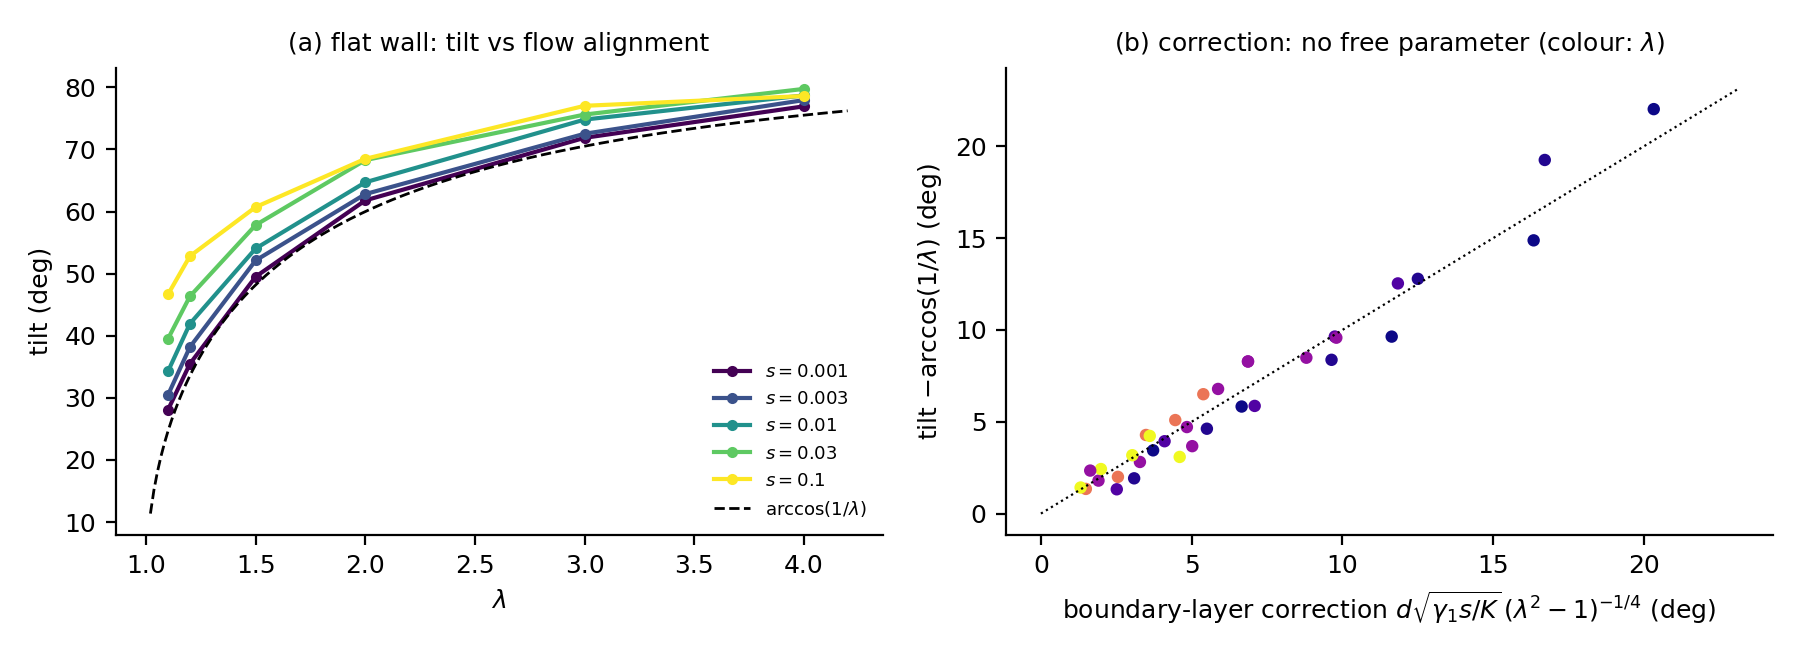
\includegraphics[width=0.9\textwidth]{fig_flatwall.png}
\caption{Flat no-slip wall in simple shear (Q-tensor). (a) Tilt vs $\lambda$ for shear rates $s$; dashed: $\arccos(1/\lambda)$, the weak-shear limit. (b) Tilt in excess of $\arccos(1/\lambda)$
against the boundary-layer correction of Eq.~\eqref{eq:tilt}, using each run's defect depth; dotted: equality.}\label{fig:flatwall}
\end{figure}

\paragraph{Mapping to MPCD.} MPCD rotates each particle by Jeffery's equation with Bretherton parameter $\lambda$ (\texttt{shearSusc} scales the rate, not the angle).
Two measurements in the passive swirl runs support the mechanism: the director at the defects' depth is rotated by 26--33$^\circ$ ($\theta_L=30^\circ$), and the tilt equals twice
that rotation (65.5 vs 63.7$^\circ$, 61.6 vs 61.0$^\circ$). Averaging Jeffery's equation over the particles of a cell suggests a reduced alignment parameter
$\lambda_\mathrm{eff}=\lambda(1+S_4)/(2S_2)$ (with $S_2=\langle\cos2\psi\rangle$, $S_4=\langle\cos4\psi\rangle$; measured particle-level $S_4$ agrees with a Maier--Saupe distribution), which
would make the tilt depend on the order parameter. \emph{It does not:} varying the mean-field potential ($U=5$, 10, 20; bulk order 0.56, 0.87, 0.94) and the density (10, 20 per cell)
gives 61.5--64.8$^\circ$ throughout (density 10/20/40: 62.4/61.5--62.2/62.6$^\circ$), while $\lambda_\mathrm{eff}$ predicts 61.5 / 56.7 / 58.2$^\circ$ (bulk order) or 68.5 / 58.7 / 57.2$^\circ$ (order near the cores).
A direct measurement of the bulk Leslie angle (sheared channel, no anchoring, no defects) shows that the MPCD alignment \emph{does} depend on the order parameter near tumbling, roughly as
$\lambda_\mathrm{eff}$ predicts ($\lambda=1.2$: 17.4$^\circ$ at $S=0.56$, 14.2$^\circ$ at $S=0.95$; $\lambda_\mathrm{eff}$: 18.9, 14.4$^\circ$), while at $\lambda=2$, $U=10$ it sits at the bare value
(29.9$^\circ$). At $\lambda=2$ the channel gives 32.8, 29.9 and 31.1$^\circ$ for $U=5$, 10, 20, following the particle-averaged prediction (30.8, 28.4, 29.2$^\circ$) with a constant offset of
$+1.8^\circ$, so MPCD does not use the bare $\lambda$. The cavity tilt equals twice the measured bulk Leslie angle to within $\pm3^\circ$ (62.2 vs 65.6, 62.0 vs 59.8, 64.8 vs 62.2$^\circ$); the
remainder grows with the order parameter, consistent with a correction such as splay $\neq$ bend compensating the order dependence of the alignment.

\paragraph{Splay $\neq$ bend.} Adding the measured anisotropy ($K_1/K_3=1.82$, same mean $K$) to the Q-tensor model breaks the zero mode. On a flat wall (free far field) the local
effect favours a large tilt (79$^\circ$ even without flow) and adds 6--8$^\circ$ at $\lambda=2$. In the disk, the bulk $+1$ also resists being twisted into a spiral (with $K_1>K_3$ the
planar, pure-bend vortex is cheapest), which cancels most of it: the net effect is $+2$ to $+3^\circ$ ($\lambda=2$: 66.6/69.3 vs 64.8/66.7$^\circ$; $\lambda=4$: 80.1/81.0 vs 78.2/78.9$^\circ$).
\begin{center}\small
\begin{tabular}{lccc}\toprule
MPCD $\lambda$ & $\arccos(1/\lambda)$ & + splay $\neq$ bend (model) & measured (passive swirl)\\\midrule
2 & 60$^\circ$ & $\approx62$--63$^\circ$ & 61--65$^\circ$ (active $\approx62^\circ$)\\
4 & 75.5$^\circ$ & $\approx78^\circ$ & 75--83$^\circ$\\
1.2 & 34$^\circ$ & $\approx37^\circ$ & 57$^\circ$ (weakly coherent, only partly ejected)\\\bottomrule
\end{tabular}
\end{center}
At $\lambda=2$ and 4 the estimate falls in the measured range. At $\lambda=1.2$ the MPCD cavity is only partly ejected and weakly coherent; the Q-tensor model in the same state
(not ejected, coherence $\approx0.5$) gives 58--68$^\circ$.

\paragraph{The tilt law across $\lambda$ in active circles (Fig.~\ref{fig:tiltlaw}).} Active MPCD circles (area 2500, natural activity) at $\lambda=0.8$--6, $k=6$ (3 seeds) and $k=4$, 8:
\begin{itemize}
  \item For $\lambda\ge2$ the overcharged state holds exactly (wall $2k-2$, bulk $+1$, tilt coherence $\ge0.99$, the circulation never reverses), and the tilt follows $\arccos(1/\lambda)$ within
        $3^\circ$: 63.0, 71.7, 74.8 and 77.9$^\circ$ at $\lambda=2$, 3, 4 and 6 against 60.0, 70.5, 75.5 and 80.4$^\circ$ ($k=6$); 71.6 and 78.1$^\circ$ at $\lambda=3$ and 6 for $k=4$; 70.0 and 77.5$^\circ$ for $k=8$ (2 seeds each).
        The leading-order law is a prediction that holds over a factor 3 in $\lambda$.
  \item Below $\lambda\approx2$ the circle state breaks down. At $k=6$: $\lambda=1.5$ gives 8.9 wall defects (bulk $+1.6$, coherence 0.76), $\lambda=1.2$ gives 8.2 ($+1.9$, 0.59), and the tumbling
        $\lambda=0.8$ gives 7.5 ($+2.3$, 0.29, reversing circulation). The same holds at $\lambda=1.5$ for $k=4$ (4.7 of 6, bulk $+1.6$) and $k=8$ (12.3 of 14, bulk $+1.85$, coherence 0.27). The threshold lies between $\lambda=1.5$ and 2.
  \item A possible link to the escape mechanism (Sec.~\ref{sec:escape}): a flow-aligned wall defect has $\cos\tau=1/\lambda$, so half of its jet points into the bulk at $\lambda=2$ and 83\% at
        $\lambda=1.2$. Weak flow alignment may leave the layer unprotected for the same reason elongated layers leak. Whether coherence or the layer fails first is not resolved yet.
\end{itemize}

\begin{figure}[H]\centering
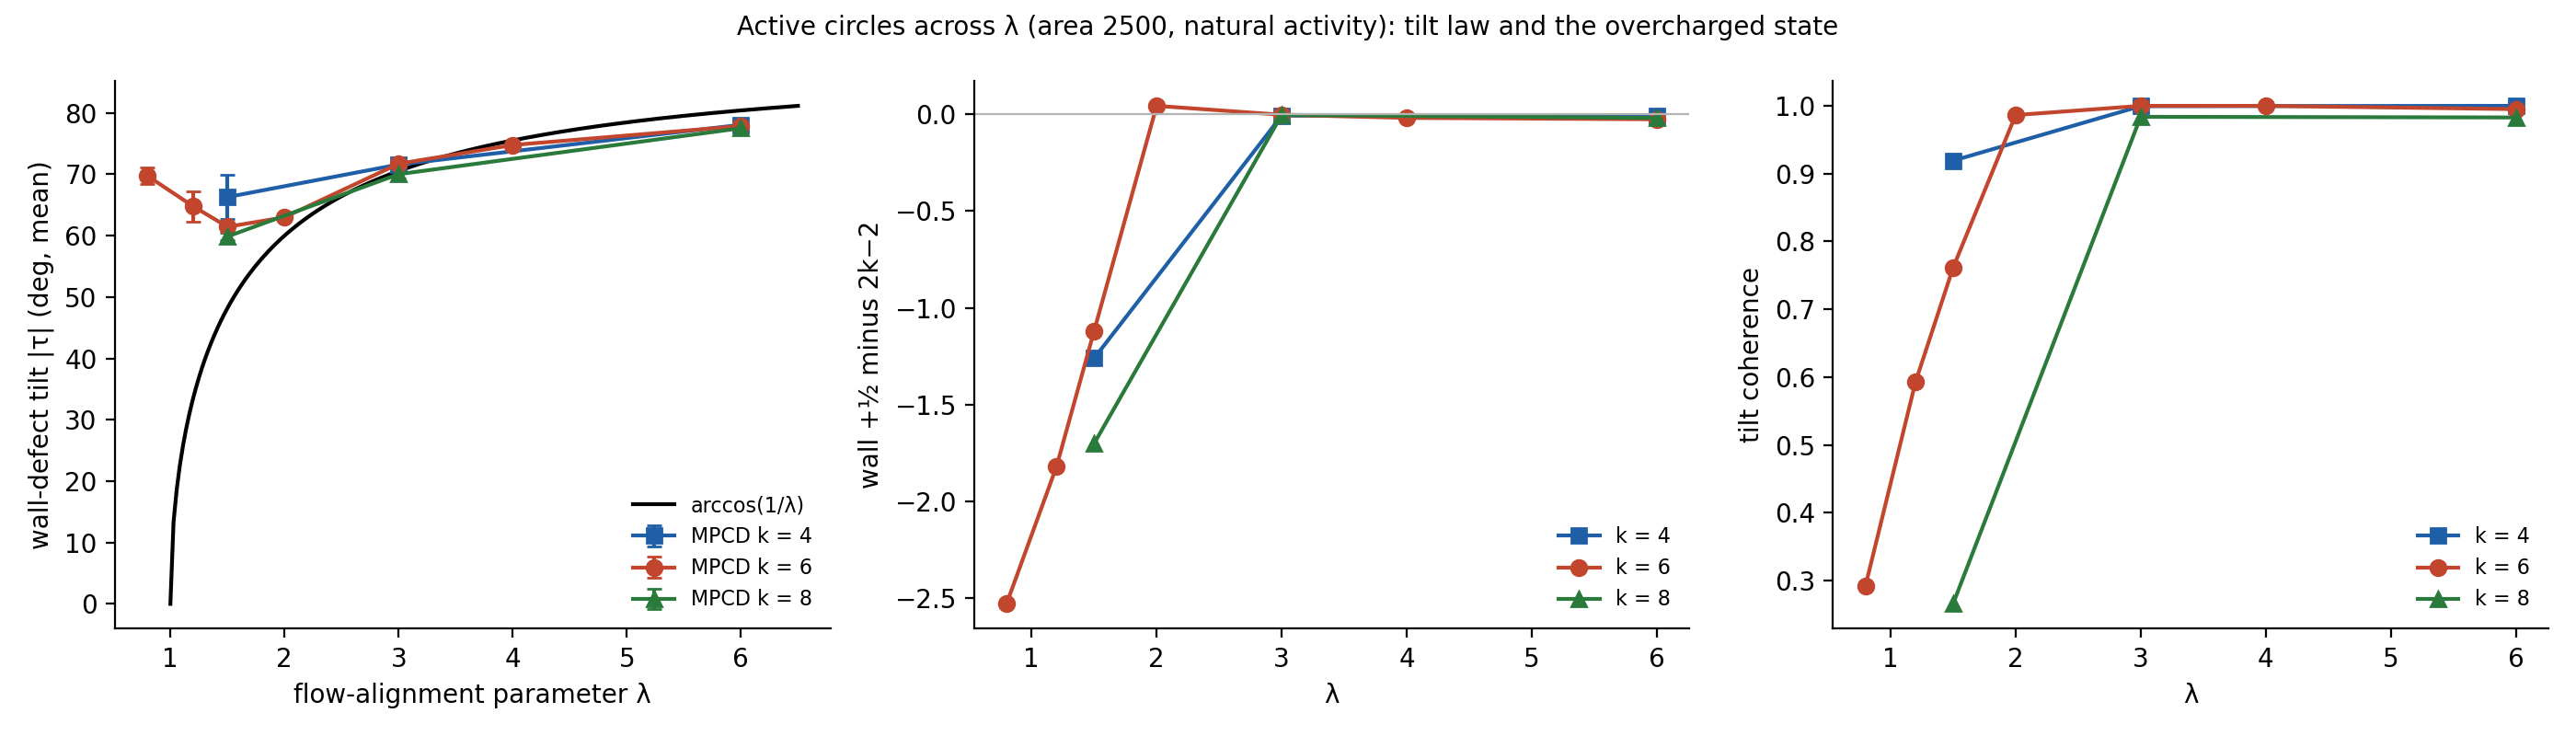
\includegraphics[width=\textwidth]{fig_tiltlaw.png}
\caption{Active MPCD circles across the flow-alignment parameter. (a) Mean wall-defect tilt against $\arccos(1/\lambda)$ (below $\lambda=2$ the layer is incoherent and the mean is not a
flow-aligned tilt); (b) wall count relative to $2k-2$; (c) tilt coherence.}\label{fig:tiltlaw}
\end{figure}

\paragraph{Not settled.}
\begin{itemize}
  \item The rotational viscosity of the MPCD nematic, from the decay of equilibrium director modes (4 seeds), is $\gamma_1\approx60\,\kT\tau/a^2$ (splay modes $62\pm2$, bend $56\pm2$),
        consistent with the measured mobility of free bulk defects ($\mu\approx0.0054$, from $\pm\half$ annihilation; wall defects: 0.02). With it, the boundary-layer correction of
        Eq.~\eqref{eq:tilt} would add $\approx16^\circ$ in MPCD, against the measured 2--5$^\circ$: the prefactor found in the continuum model does not carry over. The leading term does
        not depend on $\gamma_1$; earlier results use the measured wall-defect mobility and are unaffected.
  \item The order-dependence test above rules out the reduced order near the cores as the source of the last few degrees (an earlier version of this report proposed it).
        Density next to the wall is depleted only in the half cell at the wall and has no visible effect.
  \item Near tumbling ($\lambda=1.2$) the linear theory fails and the measured tilt is noisy (the cavity is only partly ejected).
\end{itemize}

% ======================================================================
\section{Shapes: elongation breaks the coherent flow, and the layer leaks}\label{sec:shapes}
\paragraph{One transition, set by the aspect ratio (Fig.~\ref{fig:phase}).} Tilt coherence, circulation and the single-vortex state collapse together at aspect
1.25--1.37, for ellipses and Cassini ovals alike, and at every size. The long semi-axis at the transition ranges from 1.2 to 2.3\,$\la$, so no length sets it.
\begin{itemize}
  \item Below the transition the cavity is circle-like: no vacancies, bulk $\approx+1$, coherence 0.92--0.94, one vortex.
  \item Above it: tilt coherence $\approx0.45$, two vortices 32--84\% of the time, and about 1, 3 and 4.5 vacancies at $R_\mathrm{eq}=1$, 1.5 and $2\,\la$
        (bulk charge 1.1, 1.8, 2.5).
  \item The local lock survives everywhere (0.91--0.97). What fails is the occupancy of the layer and the coherence of the flow.
\end{itemize}

\begin{figure}[H]\centering
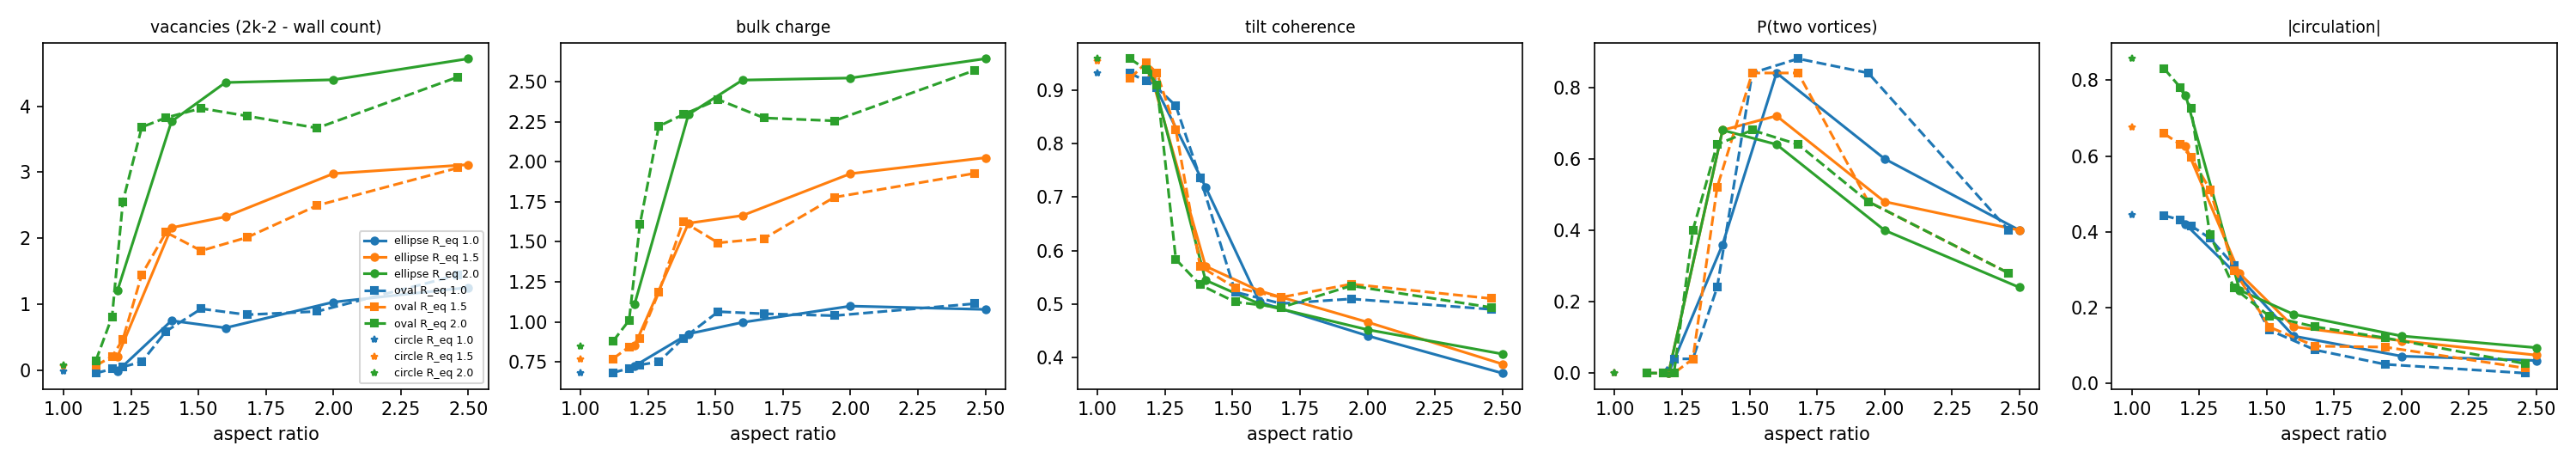
\includegraphics[width=\textwidth]{phase_shapes.png}
\caption{Shape sweep: vacancies ($2k-2$ minus wall count), bulk charge, tilt coherence, probability of two vortices and circulation against the aspect ratio. Ellipses solid, ovals dashed,
colours $R_\mathrm{eq}$; stars: circles. Medians over $k$, density and seeds.}\label{fig:phase}
\end{figure}

\paragraph{Coherent flow alone restores the circle structure in a passive ellipse.} With an imposed vortex, a passive ellipse at $\varepsilon=1.5$ goes $12\to10$ at the wall with
bulk $+1$ and a coherent tilt (0.62--0.77). Curvature therefore does not prevent the $2k-2$ layer; the ejection mechanism works in ellipses. At $\varepsilon=2$ the ejection is
partial (10--11) and the coherence lower.

\paragraph{The transition also appears in a continuum active nematic (Fig.~\ref{fig:contell}).} The active Q-tensor model with backflow (Sec.~\ref{sec:tilt}), run in ellipses of the
same area with arclength-uniform anchoring ($k=6$, $\lambda=2$, two activities), shows the same transition: circle-like for $\varepsilon\le1.2$ (10 wall defects, bulk $+1$, coherent tilt
61--62$^\circ$); above it the single vortex breaks into two, the tilt coherence drops to $\approx0.5$, and the wall loses defects to the bulk (vacancies 1--1.6 at $\zeta=0.3$, up to 4 at
$\zeta=1$, $\varepsilon=2.5$). The transition sits at $\varepsilon\approx1.4$--1.6 and moves to smaller aspect at stronger activity; at $\zeta=1$ the coherence curve nearly coincides with MPCD.

\begin{figure}[H]\centering
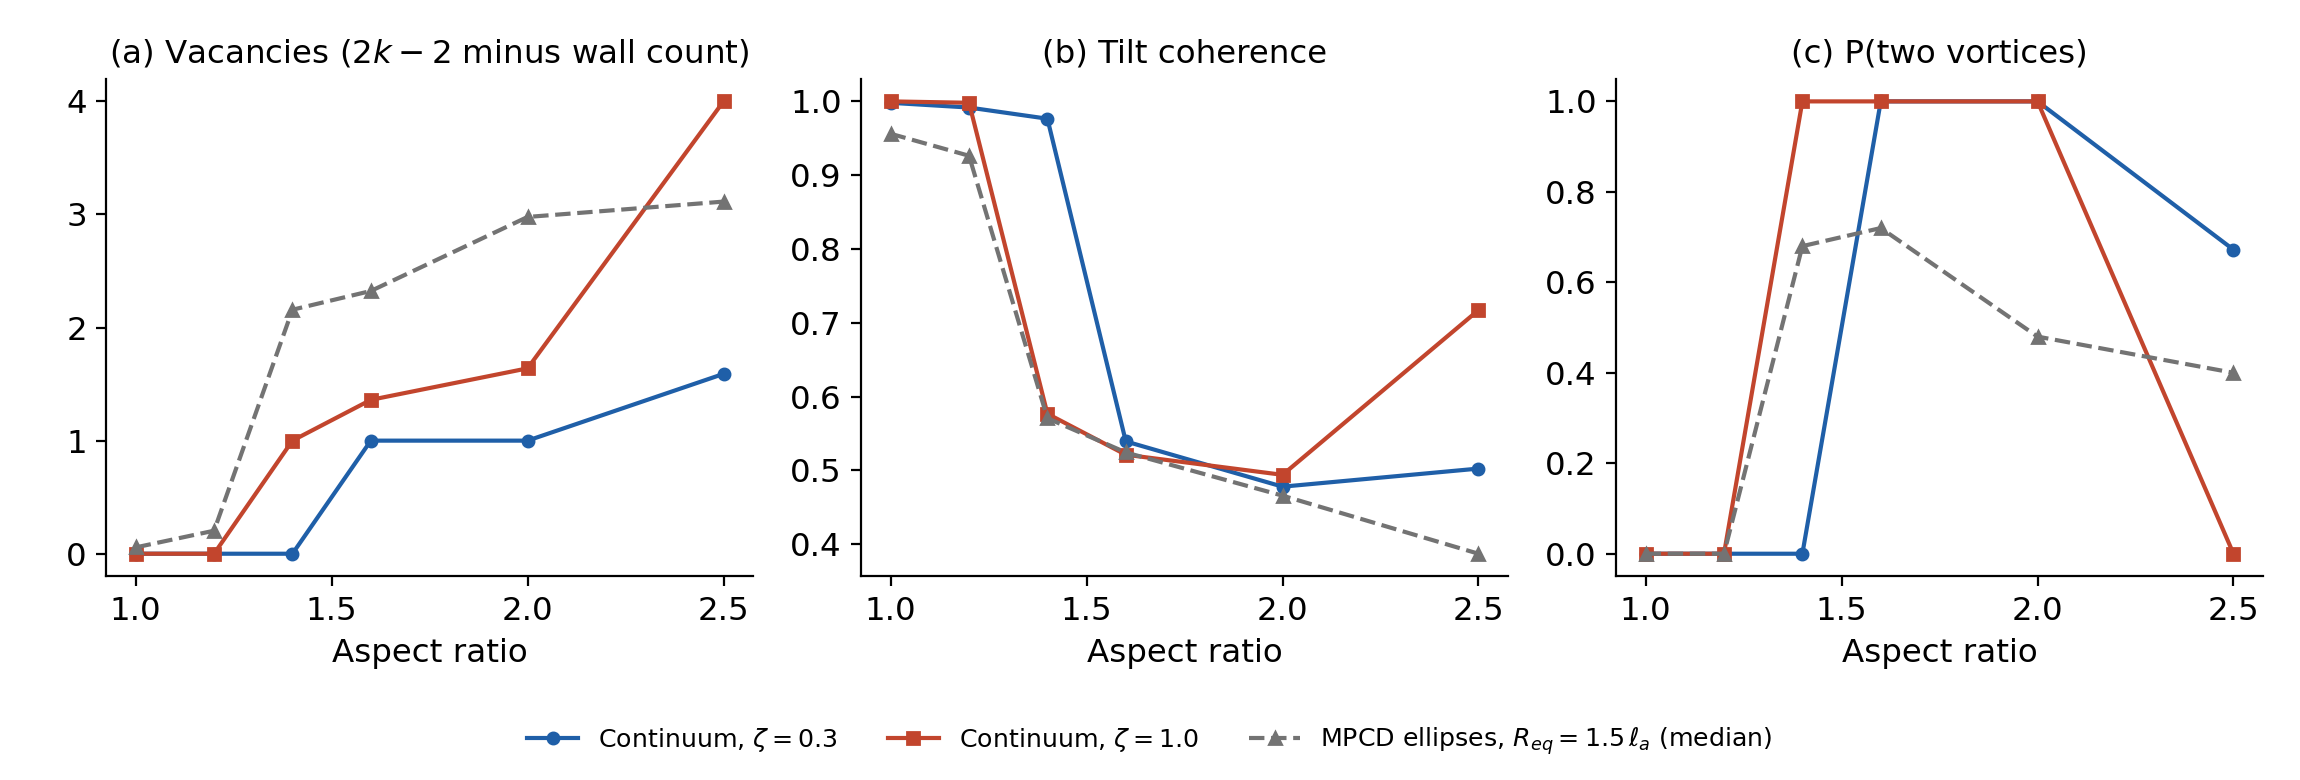
\includegraphics[width=\textwidth]{fig_cont_ellipse.png}
\caption{Active continuum model (Q-tensor, backflow, one elastic constant, $k=6$, $\lambda=2$) in ellipses of the circle's area, two activities, against the MPCD ellipse sweep at
$R_\mathrm{eq}=1.5\,\la$ (medians). (a) Vacancies; (b) tilt coherence; (c) fraction of time with two vortices.}\label{fig:contell}
\end{figure}

\paragraph{Active ellipses: what the layer loss is, and what it is not (Fig.~\ref{fig:mech}).}
\begin{itemize}
  \item \textbf{Escape-driven.} Per wall defect, escapes are 3--7$\times$ more frequent in elongated cavities at every size. At the transition they start at the tips
        (aspect 1.2: tip 0.014 vs flank 0.003 per 20\,t.u.); by aspect $\ge2$ the flanks catch up. Across runs, vacancies follow the escape rate (correlation 0.88 circle-like, 0.62 elongated).
  \item \textbf{Refill is not starved.} A bulk $+\half$ reaches the wall band equally often in every shape (ratio 0.86--1.07). But a vacancy captures it about half as
        efficiently as in a circle: net incorporation per vacancy is 0.5--0.6$\times$ the circle value.
  \item \textbf{The excess charge is free $+\half$.} Only 1--5\% of bulk $+\half$ have a $-\half$ within 4 cells (fewer in elongated cavities). The unpaired $+\half$ are not trapped at
        the tips: their mean $|x|/A$ is 0.39--0.42, as for a uniform spread. Elongated cavities also have markedly \emph{fewer} bulk $-\half$ (0.1/0.9/2.4 vs 0.4/1.9/3.9 at
        $R_\mathrm{eq}=1/1.5/2\,\la$): less pair creation in their bulk.
  \item \textbf{No cascade.} Escapes in elongated cavities are independent: a second escape right after the first is slightly \emph{less} likely than chance (0.85--0.95 at
        10--60\,t.u.). There is no excess at neighbouring sites (1.04--1.09). The per-defect escape rate does not rise as vacancies accumulate (within-run 0.89--0.98: restoring),
        and a tip escape does not raise escapes elsewhere (0.98). In the elastic model a vacancy makes its neighbours \emph{more} bound (+8--10\,$\kT$ on $\approx70$--80) and
        far sites slightly less ($-5$ to $-9$). Circles, by contrast, show mild clustering (1.1--1.7 at lag $<100$), consistent with defects being ejected two at a time.
  \item \textbf{The restoring force collapses (Fig.~\ref{fig:restoring}).} From the depth changes of 5.4 million wall-defect samples (Fokker--Planck, in units of the active noise):
        the push away from the wall is the same in both classes, but the pull back for a defect 2--3 cells deep drops from $-0.9$ to $-1.2$ (circle-like) to $-0.07$ to $-0.22$
        (elongated), and the well from 1.6--2.5 to 0.36--0.73 (tips weakest, 0.42). The noise is similar: elongated cavities hold their wall defects more weakly, they do not push harder.
  \item \textbf{Depth and self-propulsion account for a fifth.} Elongated-cavity defects sit slightly deeper (1.44 vs 1.37 cells; twice as many 3--4 cells deep), and escape rises
        steeply with depth; their self-propulsion is visible (inward drift grows with the inward head component), but on average their heads point \emph{less} into the bulk.
        With circle-like escape rates at the same depth and orientation, these differences explain 21\% of the excess.
  \item \textbf{Ruled out as the cause:} tilt misfit at curved sites (the lock holds at every site), static elasticity of the layer (tip wells only $\approx8\%$ shallower vs 25--35\%
        measured), and uneven site spacing (a circle with strongly modulated sites keeps its layer).
\end{itemize}

\begin{figure}[H]\centering
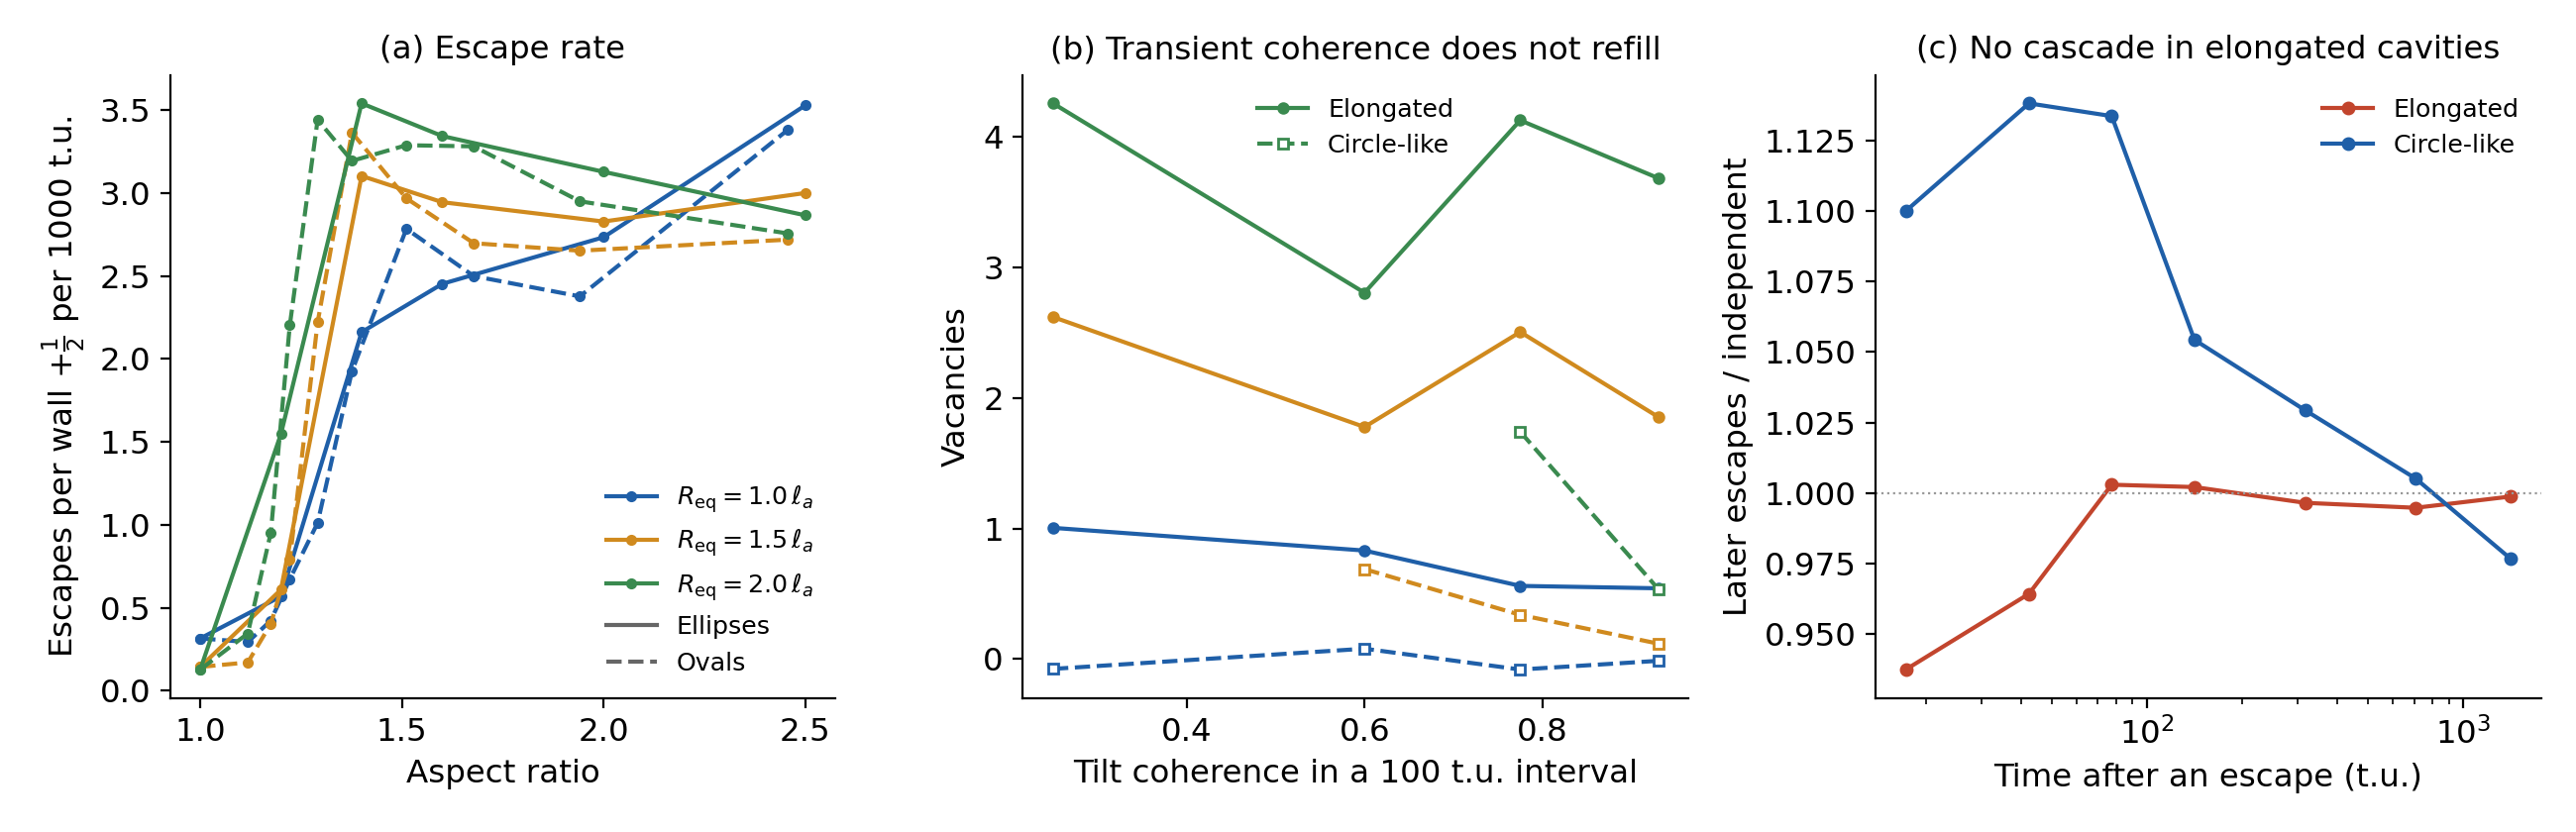
\includegraphics[width=\textwidth]{fig_shapes_mech.png}
\caption{Mechanism tests in the shape sweep. (a) Escape rate per wall $+\half$ against aspect ratio (colours $R_\mathrm{eq}$). (b) Vacancies in 100\,t.u. intervals binned by the tilt
coherence of the layer at fixed $R_\mathrm{eq}$: elongated (filled) vs circle-like (open). (c) Rate of later escapes relative to independent escapes, against the time after an escape.}\label{fig:mech}
\end{figure}

\begin{figure}[H]\centering
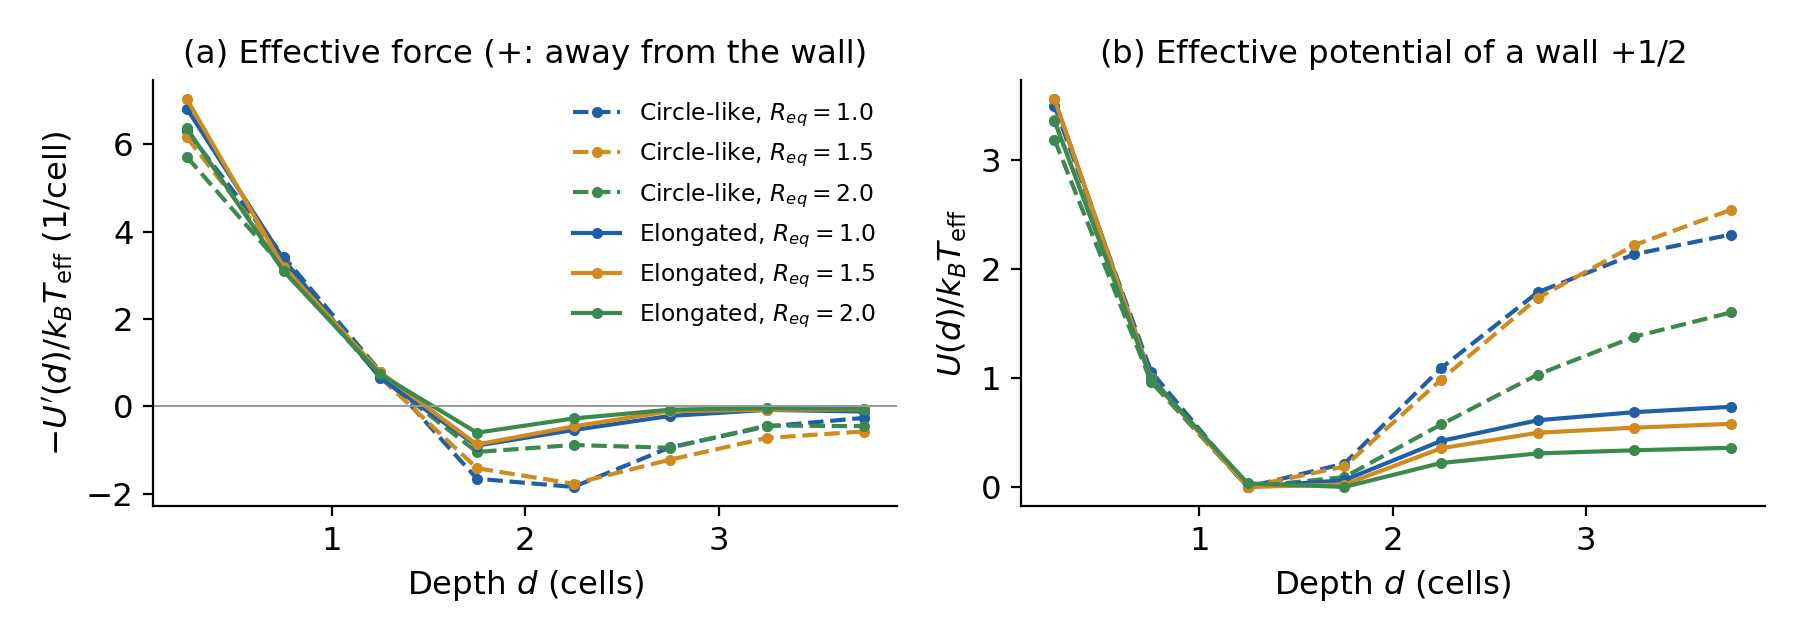
\includegraphics[width=0.9\textwidth]{fig_restoring.png}
\caption{Wall $+\half$ in the shape sweep: (a) effective force against depth and (b) effective potential, from the drift and variance of the depth change over 10\,t.u., in units of the
effective (active) noise. Dashed: circle-like cavities; solid: elongated; colours $R_\mathrm{eq}$.}\label{fig:restoring}
\end{figure}

\paragraph{Which ingredient removes the hold? Bulk activity (update 12 October).} In MPCD with no imposed flow, switching activity off everywhere except a 4-cell band at the wall keeps the
single coherent vortex, the coherent tilted layer and the full $2k-2$ wall, even at aspect 2 (wall 10.6, coherence 0.85, no two-vortex intervals), where activity everywhere gives 7.1 and
coherence 0.44. Activity only in the bulk breaks the coherence and empties the layer even in the circle (7.9, coherence 0.51). The continuum model agrees (band-only activity at aspect 2:
single vortex, 10.7 wall defects). So near-wall activity sustains the coherent near-wall circulation that tilts and protects the layer, and the elongation instability is a bulk-activity
effect. How individual wall defects then leave is the subject of Sec.~\ref{sec:escape}.

\paragraph{Open: does activity prevent the coherent flow?} B.~Loewe's hypothesis is that activity disrupts the coherent flow in elongated cavities, and the missing
coherence is what lets the layer leak. Evidence so far:
\begin{itemize}
  \item With an imposed vortex in \emph{active} ellipses (swirl up to 0.03), the layer is not repaired (wall 7--8). But the coherence only reached 0.62--0.64 (circles 0.97).
        This is not decisive.
  \item Interval statistics: at fixed size, intervals of high tilt coherence in elongated cavities still have 0.5/1.9/3.7 vacancies (circle-like: 0.0/0.1/0.5). Within a
        run, coherent intervals have only 0.1 fewer vacancies than average, whereas in circles the wall count follows coherence strongly. So \emph{transient} coherence
        (100\,t.u., 2--14\% of the time) does not refill the layer. \emph{Sustained} coherence might.
  \item \textbf{Strong imposed swirl} (0.06 and 0.1, 6--10$\times$ stronger) in active ellipses: still not repaired (wall 7.2--7.5 at $\varepsilon=1.5$, 7.3 at $\varepsilon=2$; bulk 1.7--1.95).
        Even then the tilt coherence stays at 0.63--0.65 ($\varepsilon=1.5$) and 0.35--0.37 ($\varepsilon=2$): activity keeps elongated cavities far from circle-like coherence.
  \item \textbf{Matched coherence:} the \emph{passive} $\varepsilon=1.5$ ellipse reached a similar coherence (0.62--0.77) under an imposed vortex and refilled to 10 with bulk $+1$; the
        \emph{active} one at 0.63--0.65 stays at 7.2--7.5. At the same coherence the passive layer refills and the active one does not.
\end{itemize}
So coherence matters, but activity removes wall defects by more than lowering the flow coherence; this fits the higher escape rate per wall defect found above.

% ======================================================================
% DRAFT (2026-10-12): new section on escape dynamics. To be \input after Sec. "Shapes" once the steady-state tests
% (steadyE, hazard) and the circle lambda scan are in. Numbers: RESEARCH.md entries 2026-10-11/12.
% ======================================================================
\section{How a wall defect leaves: escape dynamics}\label{sec:escape}
The shape sweep (Sec.~\ref{sec:shapes}) showed that elongated cavities lose wall defects by single escapes. Here we follow those escapes in time. We keep only
\emph{depleting} escapes: a resident wall $+\half$ (in the 4-cell wall band for at least 40\,t.u.) leaves a layer that already holds at most $2k-2$ defects, no other
defect takes its place, and the vacancy persists for 10--50\,t.u. These are the events that empty the layer. They are 11--12\% of all escapes; the rest are visitors
leaving a crowded layer or swaps. Data: the shape sweep (defects every 2\,t.u.; $\approx1640$ depleting escapes) for tilt and elastic energy, and 36 runs with flow and defects
every 2\,t.u. (area 2500, $k=6$, aspect 1--2; 411 depleting escapes) for everything involving the flow. All curves are aligned on the departure frame (escaper deeper than 6 cells within 20\,t.u.).

\paragraph{Elasticity does not let go (Fig.~\ref{fig:etsg}).} We computed the Frank energy of the measured defect configurations (point-defect model, anisotropic, cores relaxed)
with the escaper displaced along the inward normal.
\begin{itemize}
  \item The restoring force on the escaper stays at $F_0\approx-11$ to $-14\,\kT$/cell (negative pulls towards the wall) up to and through departure, at every aspect and size. It is
        indistinguishable from residents' and even grows slightly as the defect moves out.
  \item The cost of moving 6 cells in drops only in the last $\approx10$\,t.u., by 8--12\,$\kT$: that is the defect leaving, not a precursor.
  \item In elongated cavities (aspect $\ge1.4$) escape sites are elastically cheaper than residents' by 4--5\,$\kT$ from at least 40\,t.u. before (about 10\,$\kT$ at aspect 2.5; none in circles
        or at 1.2). This is a standing property of the site, about 10--15\% of the barrier, not a trigger.
\end{itemize}
So the escaper leaves against an intact elastic barrier.

\begin{figure}[H]\centering
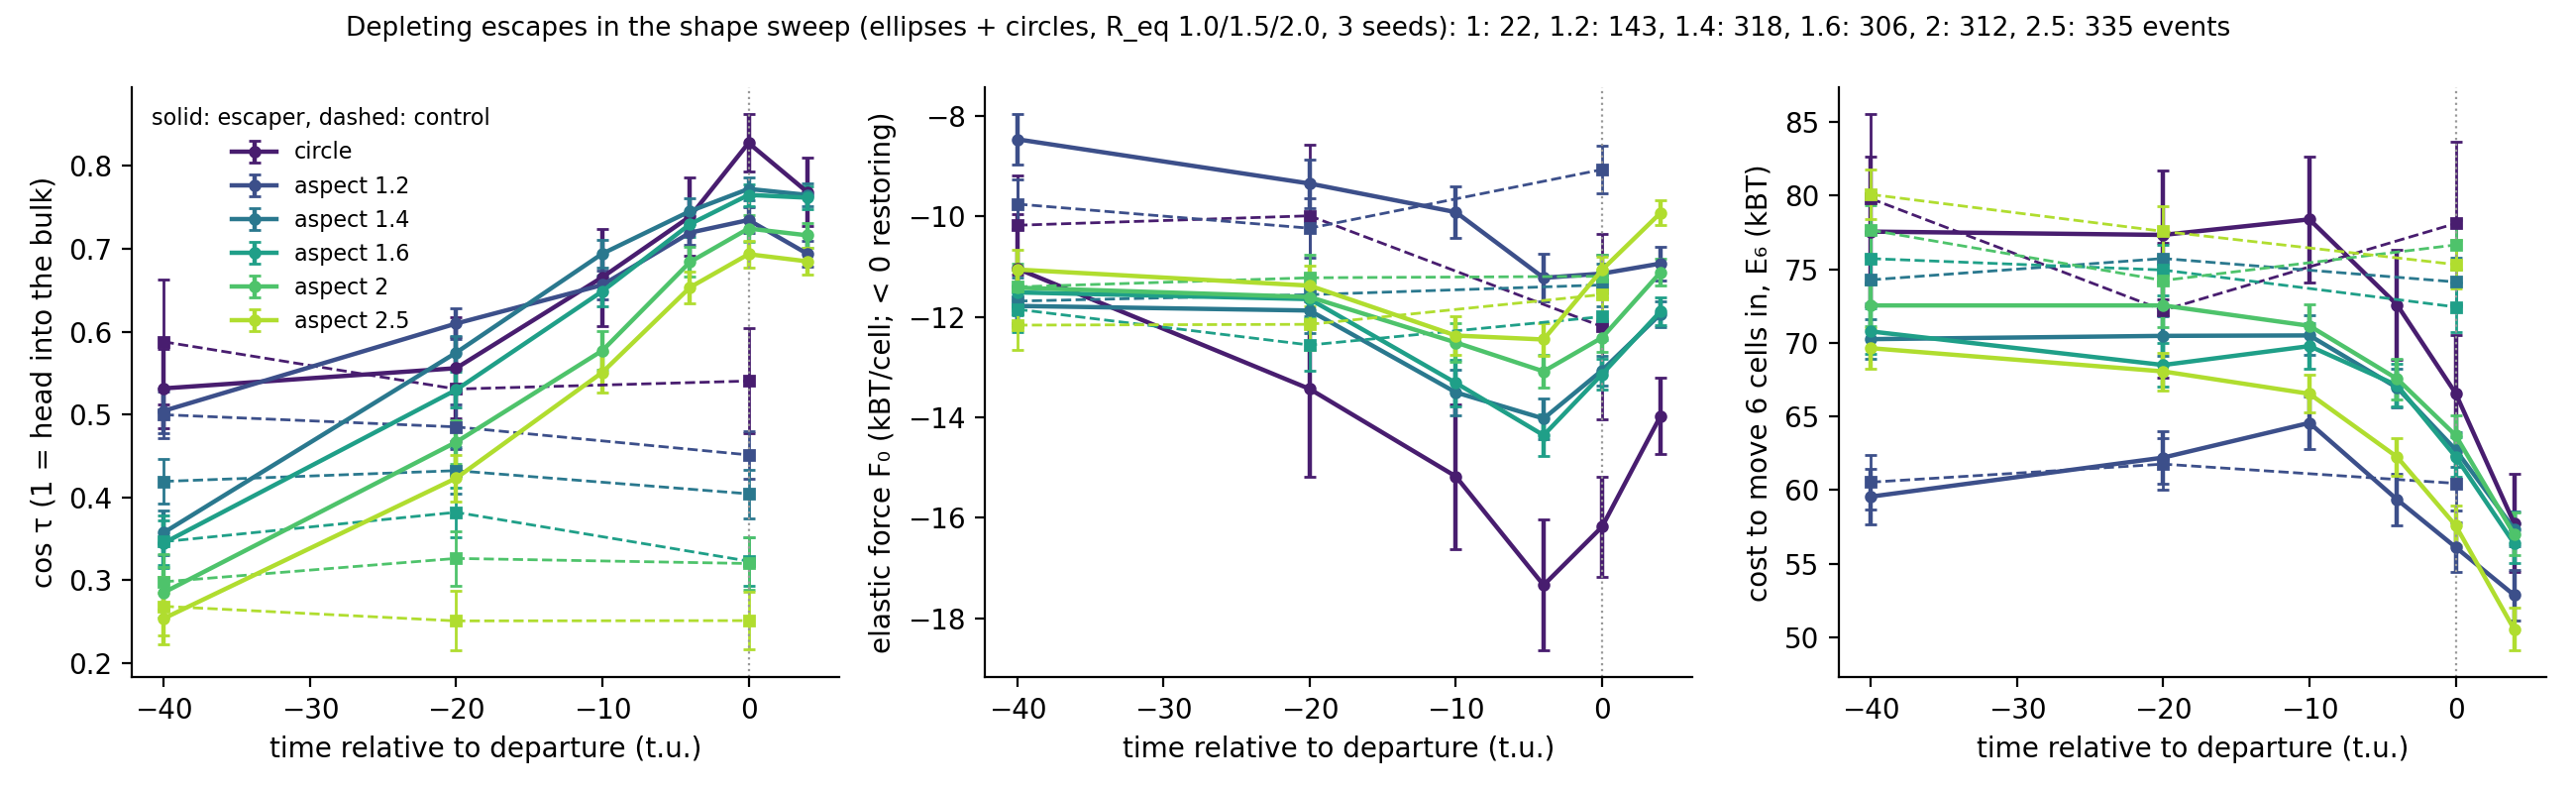
\includegraphics[width=\textwidth]{fig_etsg_shapes.png}
\caption{Depleting escapes in the shape sweep, aligned on departure, by aspect ratio (solid: escaper; dashed: random resident in the same region and frame). (a) Tilt projection
$\cos\tau$ (1 = head into the bulk); (b) elastic force $F_0$ on the defect along the inward normal ($<0$ pulls towards the wall); (c) Frank-energy cost of moving the defect 6 cells in.}\label{fig:etsg}
\end{figure}

\paragraph{Untilting first, then a local inward jet (Fig.~\ref{fig:selfflow}).}
\begin{itemize}
  \item The escaper untilts over $\approx40$\,t.u.: $\cos\tau$ rises from 0.14 at $-40$\,t.u. to 0.72 at departure, while residents stay flat. The onset is the same at every aspect and size (Fig.~\ref{fig:etsg}a).
  \item The inward flow at the defect (within 2 cells) rises only from $\approx-20$\,t.u., to 0.24 cells/t.u.\ at departure. In a ring 4--8 cells around it the flow stays flat or slightly
        \emph{outward} ($-0.01$ to $-0.02$). The burst is local to the defect.
  \item The excess flow at the core over the ring is the defect's own active jet. For free bulk $+\half$ this excess, projected on the head, is $u_\mathrm{jet}=0.32$\,cells/t.u.
        For the escaper, $u_\mathrm{jet}\cos\tau$ predicts the measured excess at departure (0.23 vs 0.24); near the wall the measured excess is $\approx0.05$ lower (see below).
  \item The defect's own inward velocity follows the flow at its core (0.08 at $-10$\,t.u., 0.34 at departure).
\end{itemize}
Untilting and the inward flow are one mechanism: the untilting turns the defect's own jet into the bulk, and the jet carries it out.

\begin{figure}[H]\centering
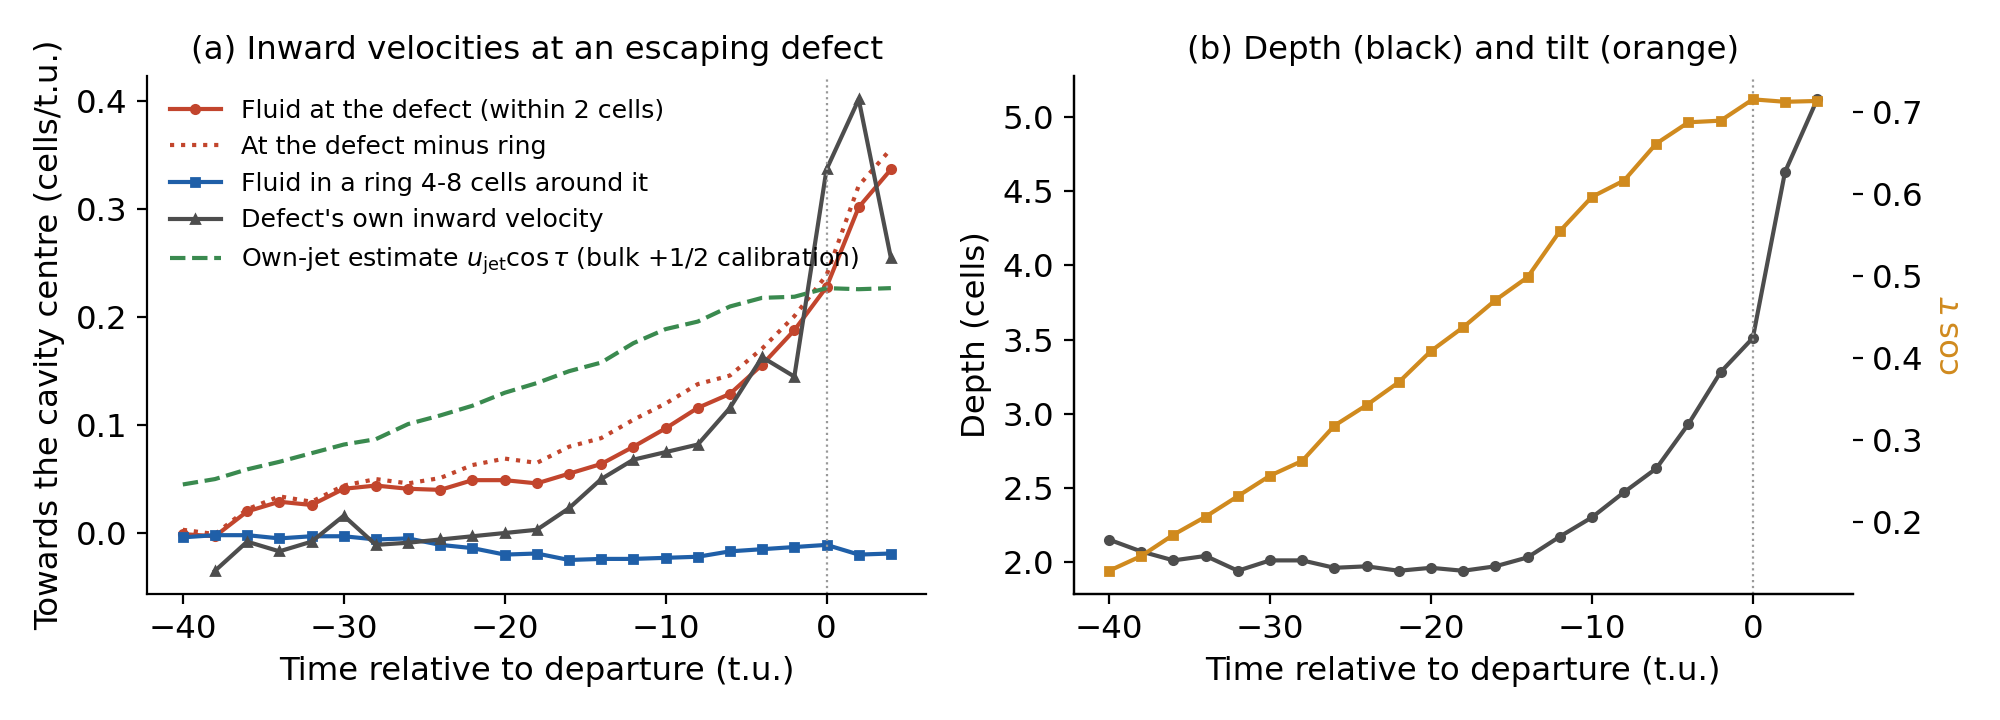
\includegraphics[width=\textwidth]{fig_selfflow_ff12.png}
\caption{Depleting escapes in the 12 fine-flow runs. (a) Inward flow (towards the cavity centre, away from the wall) at the escaper (within 2 cells), in the 4--8 cell ring, their
difference, the escaper's own inward velocity, and the own-jet estimate $u_\mathrm{jet}\cos\tau$ calibrated on free bulk $+\half$. (b) Depth and $\cos\tau$.}\label{fig:selfflow}
\end{figure}

\paragraph{The wall blocks the inward part of the jet (Fig.~\ref{fig:jetmap}).} Measured for all $+\half$ (38\,565 samples) by depth and tilt:
\begin{itemize}
  \item The jet strength along the head is \emph{not} reduced near the wall: 0.36--0.40\,cells/t.u.\ at depth 0--3 against 0.32 in the bulk.
  \item Its component along the wall normal is. The fraction transmitted, $g(d)$ (inward jet over $u_\mathrm{jet}\cos\tau$), is 0.30--0.33 within 2 cells of the wall, 0.58 at 2--3,
        0.86 at 3--4 and $\approx1$ beyond 4 cells. This is the no-penetration condition: near the wall the jet is turned along it.
  \item Closed law: inward jet $=0.40\,\cos\tau\,g(d)$. It predicts the residents' inward jet exactly (0.056 vs 0.055 at depth 2.1, $\cos\tau=0.34$).
\end{itemize}

\begin{figure}[H]\centering
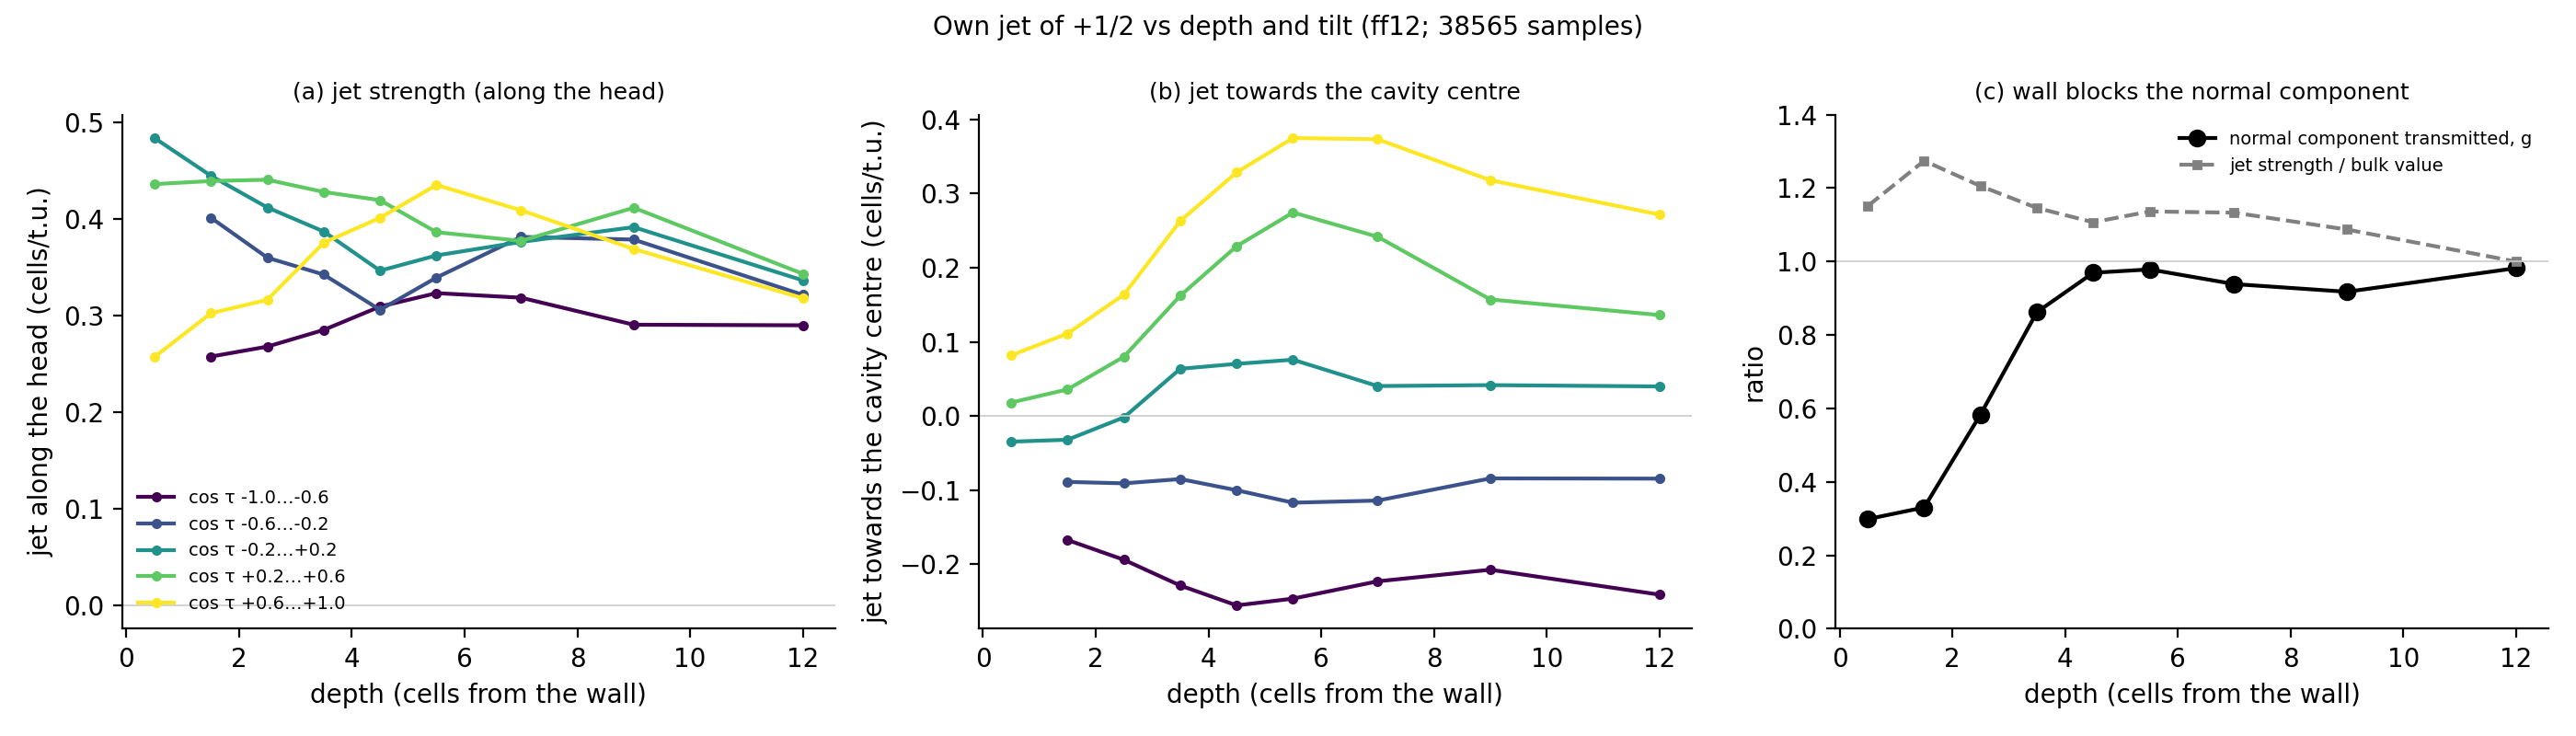
\includegraphics[width=\textwidth]{fig_jetmap_ff12.png}
\caption{Own jet of $+\half$ defects (flow within 2 cells minus the 4--8 cell ring) against depth, by tilt. (a) Strength along the head; (b) inward component; (c) transmitted fraction
of the normal component $g(d)$ and the strength relative to the bulk.}\label{fig:jetmap}
\end{figure}

\paragraph{In the flow field: the wall erases one vortex lobe (Fig.~\ref{fig:vort}).} A free $+\half$ carries two counter-rotating vortex lobes on either side of its head;
its jet is the flow between them. Measured relative to a free bulk $+\half$ (lobe vorticity 0.12/t.u.):
\begin{itemize}
  \item Near the wall the lobe on the wall side is absent: $-0.13$ of the free value at depth 1--2, 0.10 at 2--3, 0.35 at 3--4, 0.48 at 4--5, 0.60 at 5--6 and 0.78--0.86 deeper. This is the same depth scale as $g(d)$.
  \item With one lobe missing, a wall defect sits in net counter-rotating vorticity ($-0.051$/t.u.\ at depth 1--2, against $+0.02$ for bulk $+\half$).
  \item In escapers the wall-side lobe recovers \emph{before} the defect moves: 0.03, 0.08, 0.19, 0.34 and 0.46 at $-40$, $-20$, $-10$, $-4$ and 0\,t.u., and 0.7 just after departure (residents 0.07--0.14).
        At $-10$\,t.u.\ the escaper is still 2.2 cells deep, where the typical wall-side lobe is 0.10. The core vorticity of the escaper falls from $-0.033$ to $-0.003$/t.u.\ by departure (residents stay at $-0.03$): the escaper ends up riding its own symmetric flow.
\end{itemize}
Untilting swings the lobes so that the wall-side lobe leaves the wall and recovers; the dipole becomes symmetric again and the jet straightens inward.

\paragraph{Viscometric lines (Head et al., Nat.~Phys.~2024) (Fig.~\ref{fig:qcrit}).} With $\mathcal Q=\det\nabla\mathbf u$ ($=\half(\|\Omega\|^2-\|E\|^2)$ for incompressible flow; flow
smoothed over 2.5 cells, below which MPCD noise fills the cavity with $\mathcal Q=0$ lines):
\begin{itemize}
  \item MPCD reproduces their constraint. Bulk $+\half$ sit closer to $\mathcal Q=0$ lines than random points (median distance 0.85 vs 1.38 cells; large distances several times rarer).
        Bulk $-\half$ sit in rotation-dominated regions ($\mathcal Q_n=+0.26$, median distance 2.2 cells), away from the lines. Wall $+\half$ also prefer the lines (48--72\% within 1 cell vs 30--40\% for random points).
  \item Escapers land on a $\mathcal Q=0$ line as they leave: about 60\% within 1 cell until $-10$\,t.u.\ (residents 61--66\%), 89\% at departure and 91\% at $+4$\,t.u.
        Before that they pass through a rotation-dominated phase ($\mathcal Q_n=+0.10$ and $+0.13\pm0.02$ at $-20$ and $-10$\,t.u., residents $-0.06$ and 0.00), the one-sided lobe seen above.
\end{itemize}
In Head et al.'s language, an escape is the wall $+\half$ regaining the viscometric constraint of a free $+\half$. (The time course of $\mathcal Q_n$ depends on the smoothing scale;
the landing on $\mathcal Q=0$ at departure does not.)

\begin{figure}[H]\centering
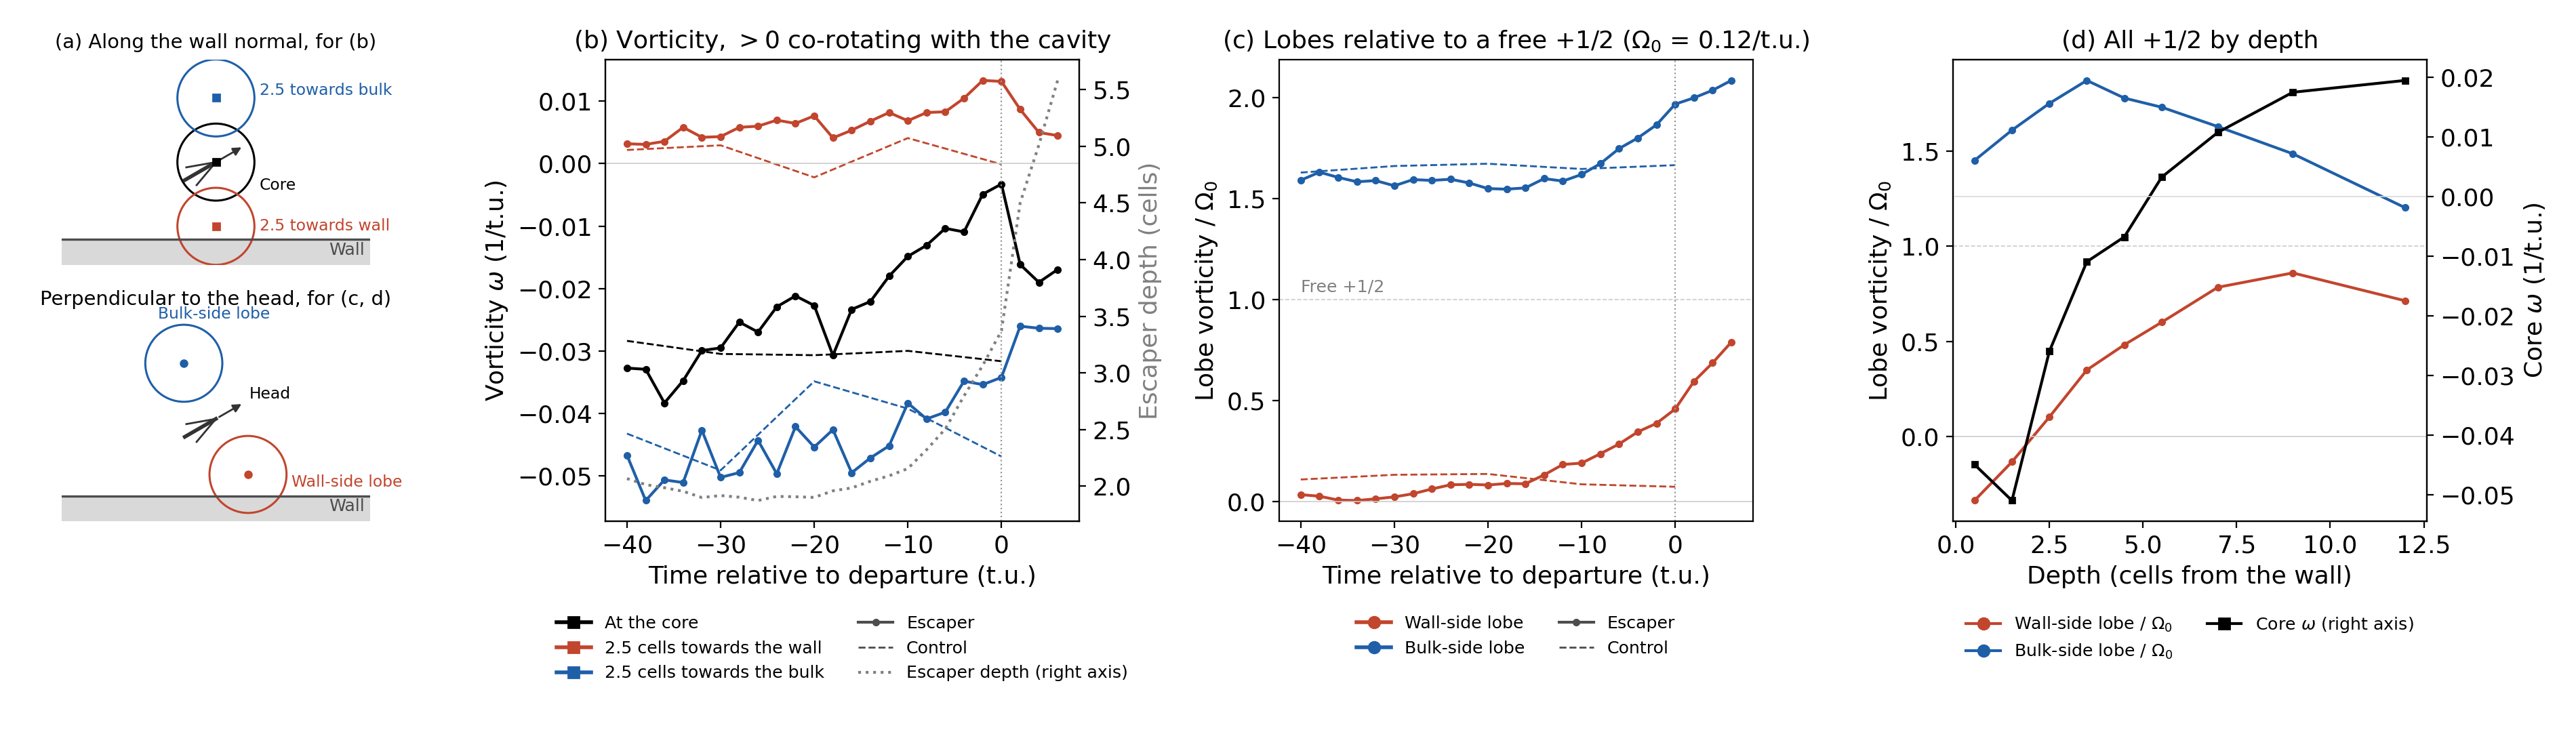
\includegraphics[width=\textwidth]{fig_vortdef_ff36.png}
\caption{Vorticity around $+\half$ defects, signed by the cavity circulation. (a) Escaper vs resident: core, 2.5 cells towards the wall and towards the bulk. (b) Strength of the escaper's
wall-side and bulk-side vortex lobes relative to a free $+\half$. (c) All $+\half$ by depth.}\label{fig:vort}
\end{figure}

\begin{figure}[H]\centering
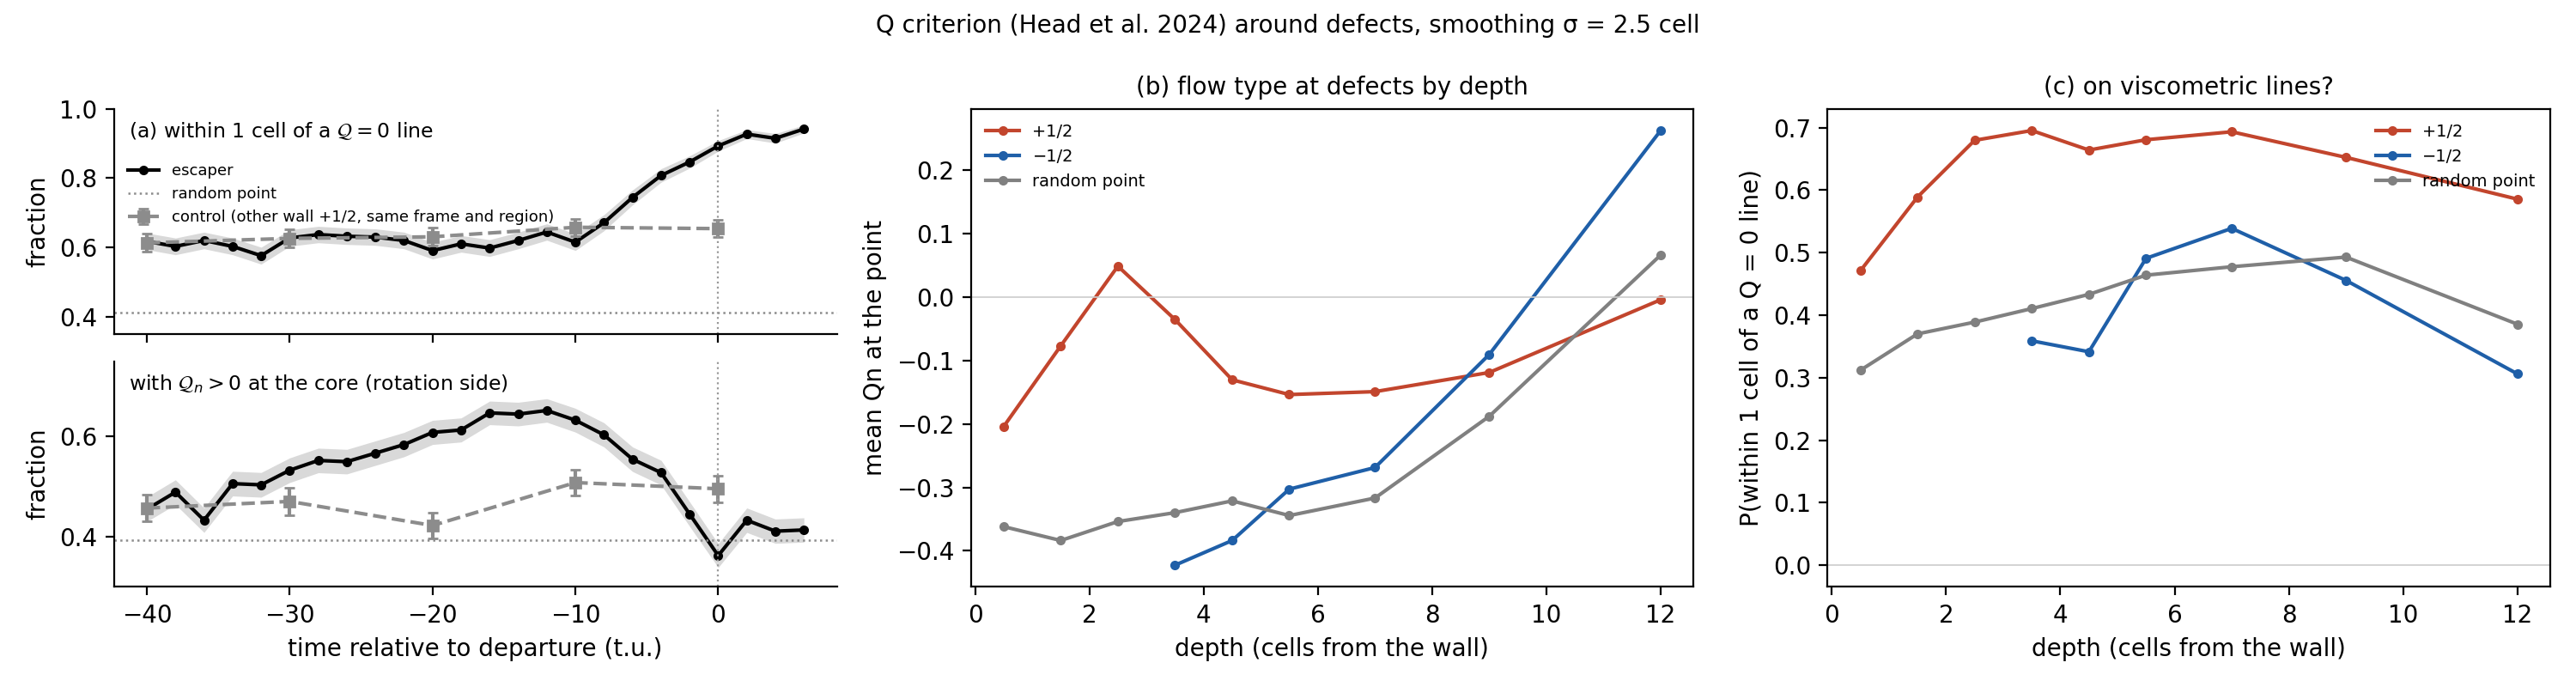
\includegraphics[width=\textwidth]{fig_qcrit_ff36s25.png}
\caption{$\mathcal Q$ criterion around defects (flow smoothed over 2.5 cells). (a) Escaper vs resident: normalised $\mathcal Q_n=(\|\Omega\|^2-\|E\|^2)/(\|\Omega\|^2+\|E\|^2)$ at the core
and the fraction within one cell of a $\mathcal Q=0$ line. (b) $\mathcal Q_n$ at $\pm\half$ and random points by depth. (c) Fraction within one cell of a $\mathcal Q=0$ line.}\label{fig:qcrit}
\end{figure}

\paragraph{Force balance.} Per frame, we fitted the escaper's inward velocity as $v_\mathrm{in}=\alpha\,u_\mathrm{jet,in}+\beta\,u_\mathrm{ring}+\mu_n F_0+c$
(own jet, background flow and elastic force, all along the inward normal; bootstrap over events):
\begin{itemize}
  \item Free bulk $+\half$: $\alpha=0.64\pm0.01$, $\beta=0.58\pm0.01$. Escapers (36 runs): $\alpha=0.87\pm0.02$, $\beta=0.98\pm0.05$, and a normal mobility $\mu_n=0.0016\pm0.0004$\,cells$^2$/($\kT$\,t.u.).
        That is about 3$\times$ below the free-defect mobility (0.0054) and more than 10$\times$ below the along-wall mobility from layer fluctuations (0.02--0.03). Treat $\mu_n$ as a lower estimate:
        $F_0$ varies little and is noisy, which biases it down.
  \item The elastic pull is therefore a drift of only $\mu_nF_0\approx-0.02$\,cells/t.u.
  \item Budget of the run-up, measured inward velocity vs model (jet, ring, elastic):
\end{itemize}
\begin{table}[H]\centering\small
\begin{tabular}{@{}rccccc@{}}\toprule
lag (t.u.) & measured $v_\mathrm{in}$ & model & jet & background & elastic \\ \midrule
$-20$ & 0.01 & 0.03 & 0.06 & $-0.03$ & $-0.02$ \\
$-10$ & 0.06 & 0.06 & 0.09 & $-0.02$ & $-0.02$ \\
$-4$  & 0.14 & 0.12 & 0.14 & $-0.01$ & $-0.02$ \\
0     & 0.36 & 0.18 & 0.19 & 0.00 & $-0.02$ \\
$+6$  & 0.31 & 0.31 & 0.33 & $-0.02$ & $-0.02$ \\ \bottomrule
\end{tabular}
\end{table}
\noindent The model tracks the run-up and misses the burst at departure, probably position jumps in the defect detection at the band edge. With the closed jet law instead of the measured jet
(tilt and depth only) the fit is somewhat worse ($R^2$ 0.21 vs 0.30) with the same $\mu_n$, and it predicts the residents' inward jet exactly (0.044 vs 0.044).

\keybox{\textbf{Escape in one paragraph.} A wall $+\half$ is held mainly by its tilt and by the wall, not by elasticity. Its jet is full strength, but the tilt points it along the wall and the
no-slip wall erases its wall-side vortex lobe, so only $\approx30\%$ of the inward component acts (about $+0.05$\,cells/t.u.). That is balanced by an elastic drift of
$\approx-0.02$ and by pinning. Untilting raises the inward projection and lets the missing lobe recover; each cell of depth then lets more of the jet act (0.33, 0.58, 0.86, 1), so the push
triples between 2 and 4 cells and the defect runs away. It leaves on a $\mathcal Q=0$ line, like a free $+\half$.}

\paragraph{Tips and flanks (Fig.~\ref{fig:etsgreg}).} Per resident wall defect, the tips leak 2--2.5$\times$ faster than the flanks at aspect $\ge1.4$. At the onset (aspect 1.2) escapes are almost only at the tips (61 vs 5 on the flanks).
From aspect 1.4 on every region leaks, and only $\approx40\%$ of escapes are at the tips. All regions share the untilting run-up, but the weak spot differs:
\begin{itemize}
  \item At the tips the whole layer is less tilted (residents $\cos\tau=0.46$ vs 0.25--0.29 elsewhere), so every tip defect already has more of its jet pointing inward. There is no elastic difference
        (escape cost 73.5 vs 75.9\,$\kT$).
  \item On the flanks and mid sections, escapes start from elastically cheaper sites: 7--9\,$\kT$ below residents from 40\,t.u.\ before, probably a gap in the layer next to the site.
  \item In the flow (36 runs: 190 tip, 140 mid, 81 flank escapes) the mechanism is the same everywhere: jet coefficient 0.82--0.90, the wall-side lobe recovers in the same way, and 87--91\% land on a $\mathcal Q=0$ line.
        At the tips the elastic pull is dynamically absent ($\mu_n=0.0005\pm0.0005$ vs 0.0024--0.0027 elsewhere) and the background flow is carried fully.
\end{itemize}

\begin{figure}[H]\centering
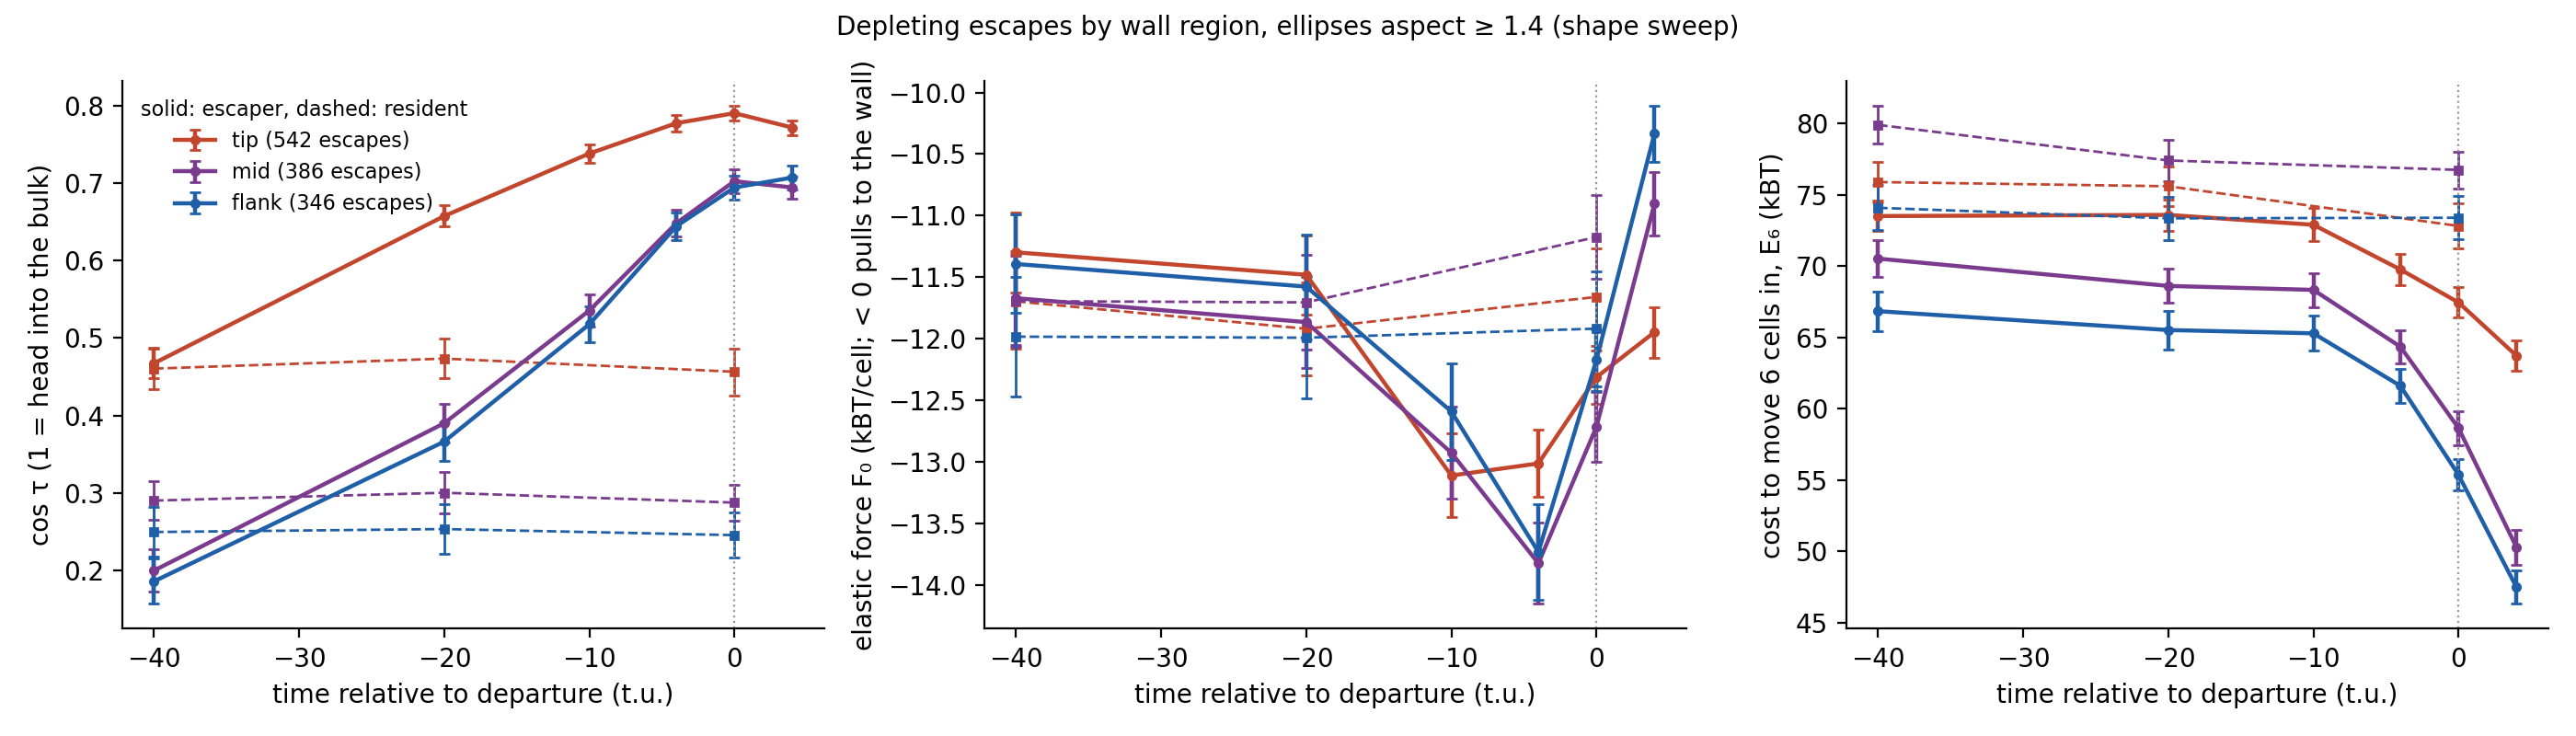
\includegraphics[width=\textwidth]{fig_etsg_reg.png}
\caption{As Fig.~\ref{fig:etsg}, by wall region (tip, mid, flank by the ellipse angle parameter), pooled over aspect $\ge1.4$.}\label{fig:etsgreg}
\end{figure}

\paragraph{Ovals.} The same analyses on the Cassini ovals of the shape sweep (405 runs) and on 12 oval runs with fine flow output (aspect 1.5 and 1.9) give the same
picture: the same untilting precursor at every aspect, the same tip weakness through a less tilted tip layer, the same crowding feedback, the own jet matching $u_\mathrm{jet}\cos\tau$ at
departure, the same lobe erasure and recovery (wall-side lobe 0.08, 0.20, 0.55 at $-20$, $-10$ and 0\,t.u.), and the same landing on $\mathcal Q=0$ lines (92\% at departure). With the elastic model rebuilt for Cassini walls, a depleted oval layer is equally far above its elastic optimum: refilling the largest gap lowers the Frank energy by 81--89\,$\kT$ at aspect 1.4--1.9. Two small
differences: within 2 cells of the wall slightly more of the jet gets through ($g\approx0.45$ vs 0.3), and the mid section of an oval leaks about as much as its tips.

\paragraph{A second route: active bulk, passive wall (Fig.~\ref{fig:bulkonly}).} With activity switched off within 4 cells of the wall (10 runs, same fine output), the layer still empties,
even in circles (0.2--1.0 depleting escapes per wall defect per 1000\,t.u.; the active circle has none). The escape kinematics look the same, but what accompanies them does not:
\begin{itemize}
  \item The wall band is quiet and strain-dominated: wall circulation 0.016--0.03 (active 0.13), $\mathcal Q_n=-0.5$ to $-0.65$ (active $\approx0$).
        A $+\half$ in the passive band keeps 20--28\% of its jet and almost no lobes.
  \item There is no untilting precursor ($\cos\tau\approx0.2$ until $-20$\,t.u.; it turns only during the motion), no own jet in the band, and the background flow is slightly \emph{inward}.
  \item The force fit leaves an unexplained inward drift ($c=+0.05\pm0.014$), possibly noise plus the selection of events.
\end{itemize}
So without wall activity there is no protection and no jet: defects drift out of a quiet wall with the background flow and fluctuations against the weak elastic hold. This route
exists only when the coherent active wall circulation is absent. It is how bulk-only activity empties the layer even in circles.

\begin{figure}[H]\centering
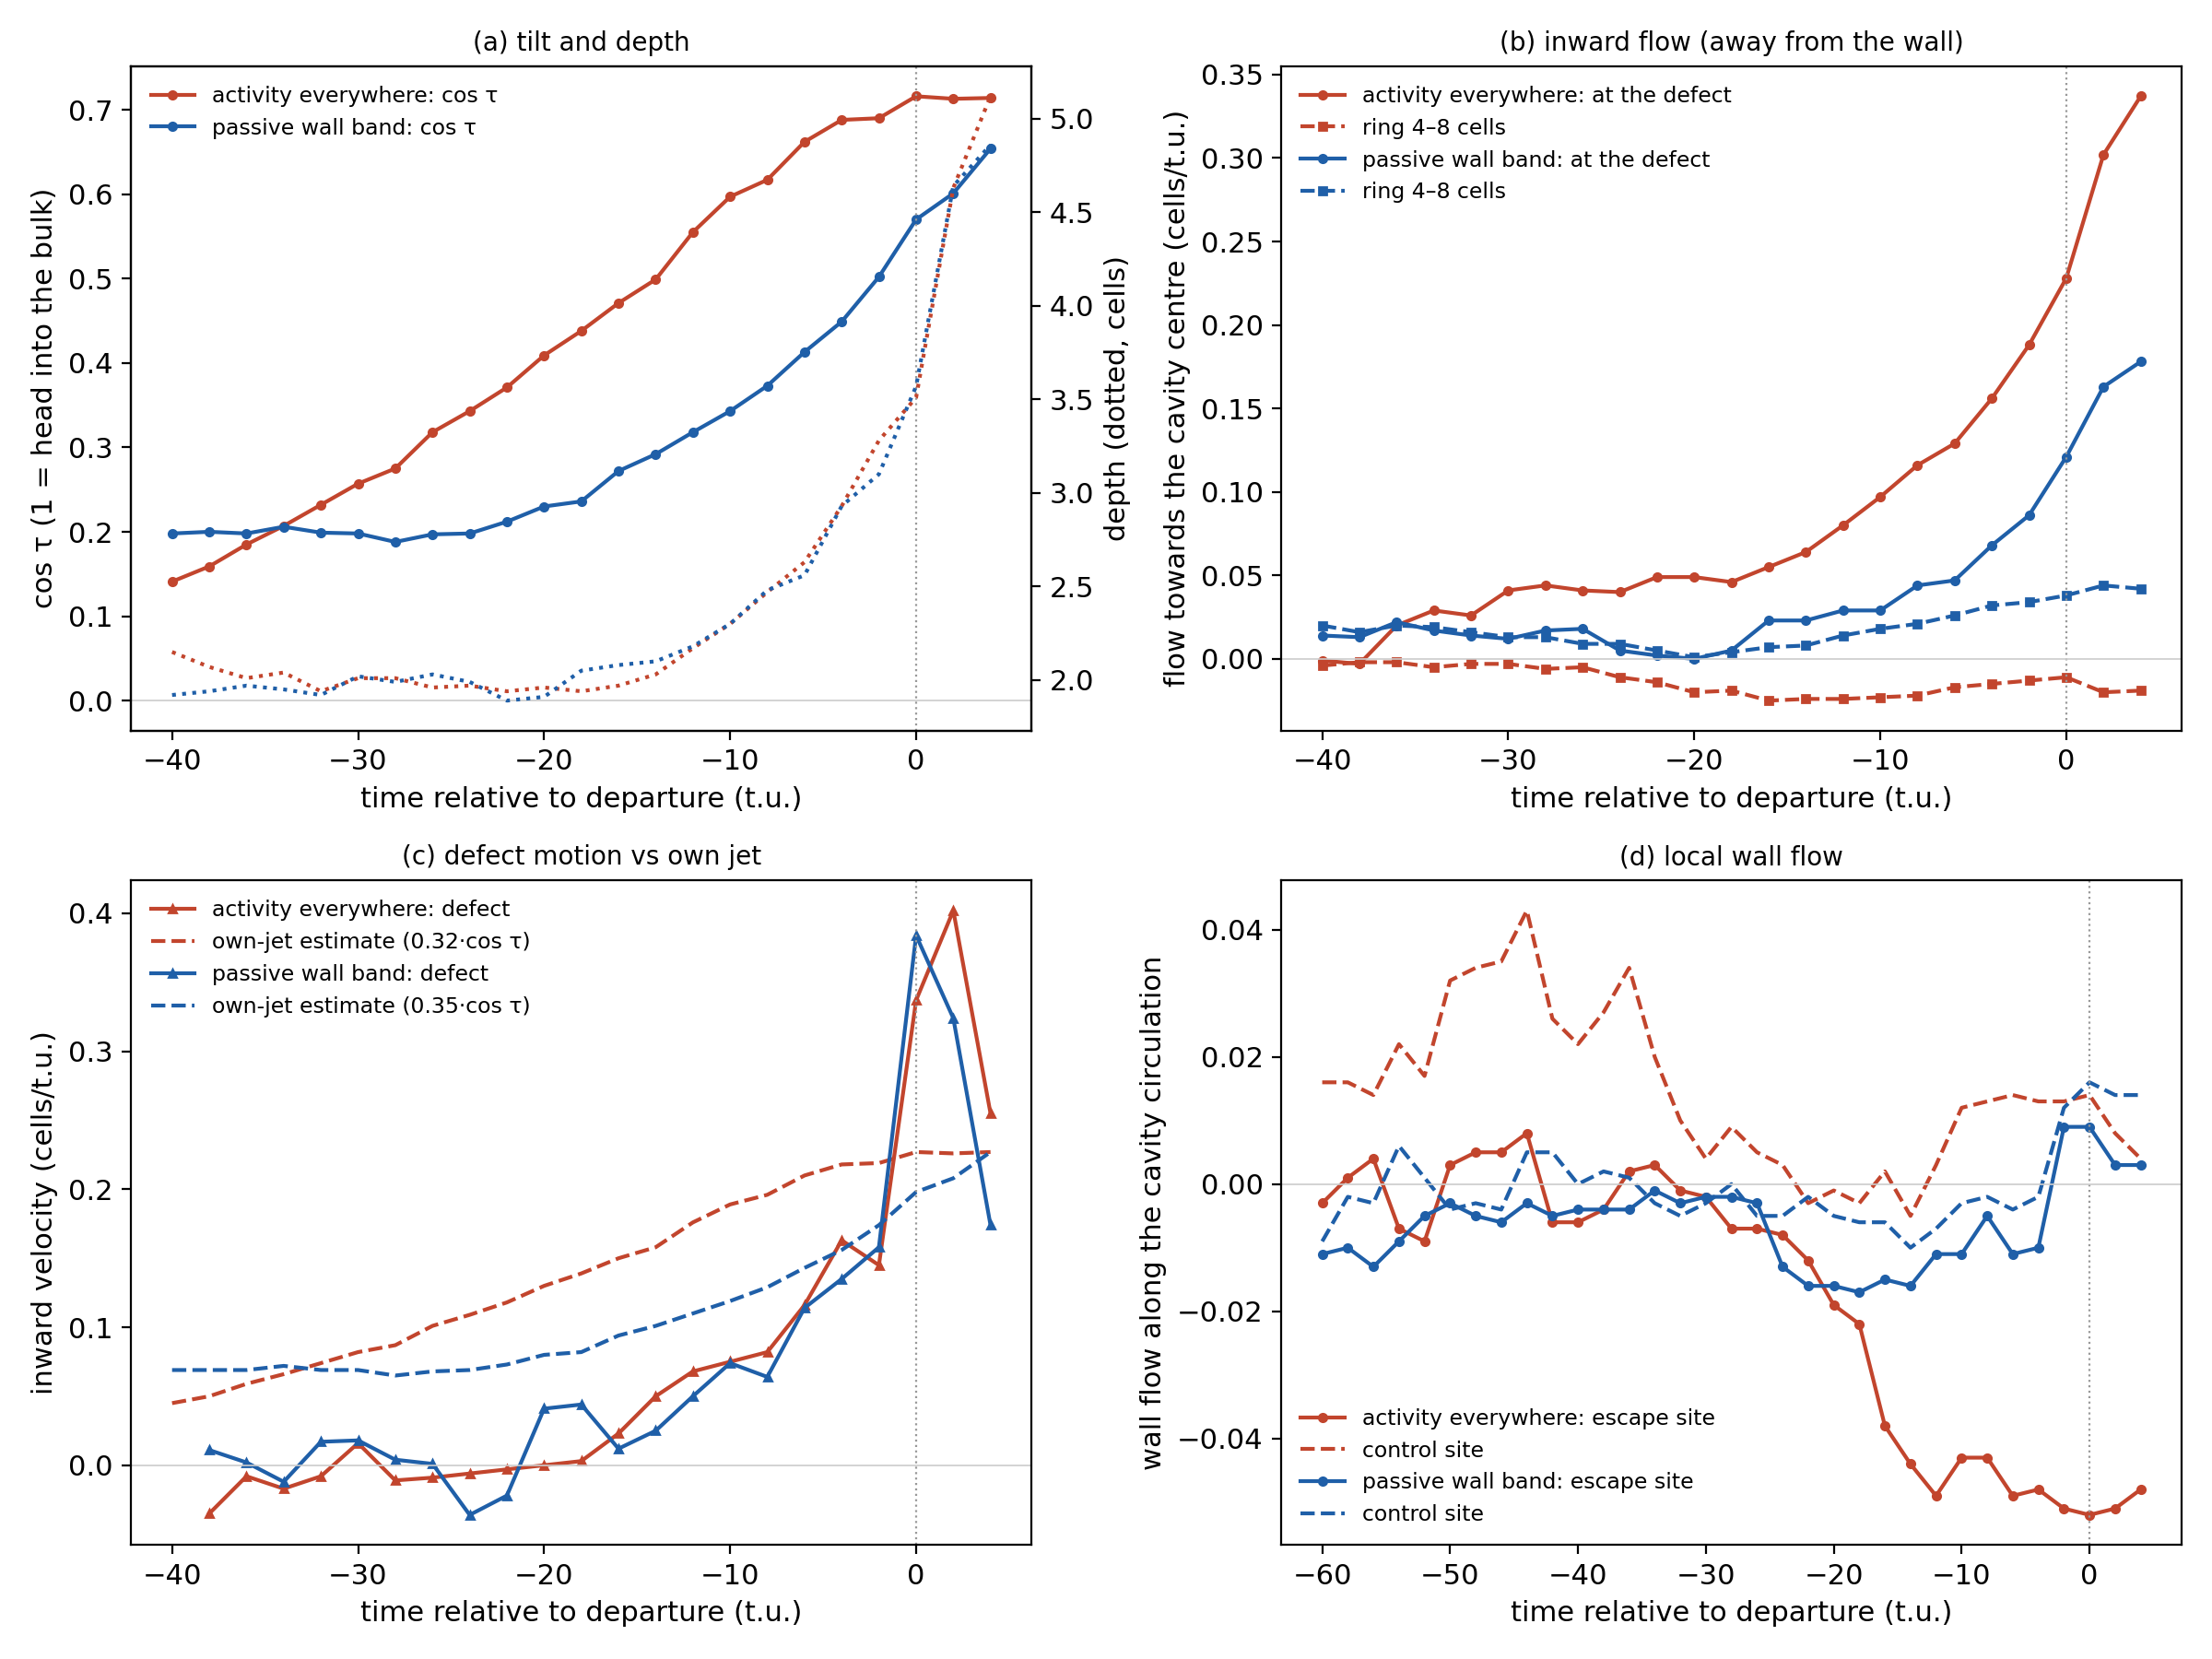
\includegraphics[width=0.85\textwidth]{fig_compare_bulk.png}
\caption{Depleting escapes with activity everywhere (red) vs activity only beyond 4 cells from the wall (blue). (a) Tilt and depth; (b) inward flow at the defect and in the 4--8 cell
ring; (c) the defect's inward velocity and the own-jet estimate; (d) local flow along the wall, signed by the cavity circulation, at the escape site and at a control site.}\label{fig:bulkonly}
\end{figure}

\paragraph{Rates are not the steady state: the $\lambda$ test.} Changing the flow-alignment parameter changes the tilt, and with it the escape rate, as the mechanism predicts. In the
aspect-2 ellipse, going from $\lambda=1.2$ to 2 to 4, the residents' $\cos\tau$ falls (0.24, 0.19, 0.14) and the depleting-escape rate falls 15$\times$ (1.01, 0.65, 0.066 per wall
defect per 1000\,t.u.). The flow gets \emph{stronger} with $\lambda$ ($v_\mathrm{rms}$ 0.46, 0.57, 0.70), so this is not a weaker-flow effect. But entries slow too: from $\lambda=2$ to 4
exits drop 6$\times$ and refills of a vacancy 3.7$\times$. The wall count barely moves (7.1, 7.1, 7.65 instead of 10). The tilt and the jet blocking set how fast defects cross the wall band
in both directions; they do not set how many the wall keeps. At $\lambda=1.2$ even the circle loses the overcharged state (wall 7.9, bulk $+2.05$, wall circulation a third of $\lambda=2$).

\paragraph{What sets the steady state? A dynamical balance far from the elastic optimum.}
\begin{itemize}
  \item \textbf{The depleted layer is not an elastic minimum.} In measured steady-state configurations, moving one bulk $+\half$ into the largest wall gap \emph{lowers} the Frank
        energy by 80--100\,$\kT$ in elongated cavities (median of the best mover; favourable in 75--100\% of frames), while ejecting a wall $+\half$ costs 50--85\,$\kT$.
        Even in the circle an extra wall defect is favourable ($-28\,\kT$), as expected since passive cavities keep all $2k$ at the wall. The overcharged bulk ($+1$ in circles,
        $+2.2$ to $+2.5$ in elongated cavities) is held up by the active dynamics against a large elastic preference for a full wall. (The passive point-defect model ignores the active tilt.)
  \item \textbf{The bulk charge limits itself through the exits} (B.~Loewe's hypothesis). Within runs (49 elongated runs, $\approx195\,000$ wall-defect frames), when the bulk charge is
        above its run average the wall defects exit less often: relative to the average, 1.9$\times$ at one unit below and 0.9$\times$ at one unit above.
        \begin{itemize}
          \item Not through the jet: the wall defects sit closer to the wall (0.12 cell per unit of charge), but they are also less tilted, so their inward jet push is unchanged.
          \item Not through bulk pressure: the push of the bulk charges on wall defects (2D defect interaction) is the same at tips, mid and flanks at every aspect, and adding it to the
                per-defect model explains little.
          \item \emph{Through the crowding of the layer.} The exit rate per wall defect falls as the layer empties: 0.068 per 20\,t.u.\ for a full layer of $2k-2$, 0.050, 0.037 and 0.028 with one,
                two and five vacancies. With crowding included the per-defect model reproduces most of the trend. A sparser layer holds its remaining defects more strongly; in the
                elastic model a vacancy makes its neighbours more bound by 8--10\,$\kT$. As the bulk charges up, the wall empties and each remaining wall defect sits in a deeper well.
        \end{itemize}
  \item \textbf{Refill.} Entries per vacancy fall with the bulk charge, but the total entry flux rises (0.11$\to$0.39 per frame), because vacancies grow faster. Both fluxes are restoring.
        Refill is slowed by the same tilt and jet blocking as the exits (the $\lambda$ test).
  \item \textbf{The steady state is unique.} Runs seeded with 10, 7 or 4 wall defects (aspect 2, $k=6$, 4 seeds each, seeding through a new initial-director option) all converge to
        $7.2\pm0.1$ wall defects and bulk $+2.4$ within 300--700\,t.u., the value of unseeded runs. Circles seeded with 12 (the passive arrangement) or 6 wall defects both end at $2k-2=10$ with bulk $+1.0$.
\end{itemize}
The steady state sits where an exit flux that falls as the layer empties meets a refill flux that rises with the vacancies, far above the elastic optimum. The tilt sets how fast both
fluxes run; the geometry (through the coherence of the flow) sets where they cross.
% TODO after runs/lambda_circle: tilt law across lambda in active circles, and the lambda range where the circle state survives (lambda 1.2 already loses it).


% ======================================================================
\section{Current picture and open questions}
\begin{table}[H]\centering\small
\begin{tabularx}{\textwidth}{@{}lX@{}}
\toprule
\textbf{Established} & $(2k-2)$-fold anchoring symmetry; tilt--position lock; pinning of the commensurate ring by $K_1\neq K_3$; passive registry set by the initial condition;
flow-induced ejection (energetics and passive imposed-flow test, $\lambda$ dependence); bulk drives the flow, layer brakes it; shape transition at aspect 1.25--1.37, scale-free (reproduced by the active continuum model);
layer loss in elongated cavities is escape-driven and non-cascading; the tilt--position lock as the zero mode of the layer; the tilt $\arccos(1/\lambda)$ from flow
alignment in the no-slip shear (continuum model, flat-wall theory, and active MPCD circles for $\lambda=2$--6); near-wall activity alone sustains the coherent state, bulk activity breaks it;
escape mechanics: intact elastic barrier, untilting first, own jet turned along the wall and blocked by the wall ($g(d)$), wall-side lobe erased, landing on $\mathcal Q=0$ lines;
stronger alignment slows exits and refills alike; the overcharging of elongated cavities follows a wall law, bulk charge $\approx c(q)\times$ perimeter, the same in ellipses, ovals and channels. \\
\textbf{Supported} & Layer as an effective planar winding-1 boundary with a spiral feedback, giving the onset $R/\la\approx0.4$--0.6; bulk $+1$ as the charge enclosed
by that boundary; splay $\neq$ bend and the boundary layer supply the remaining few degrees of tilt at $\lambda=2$; force balance with a small normal mobility ($\mu_n\approx0.002$);
the steady wall population as a unique dynamical balance (seeded starts converge) far from the elastic optimum, self-limited by layer crowding; ovals behave as ellipses at the escape level (defect, flow, vorticity and $\mathcal Q$ signatures); tips weaker through their lower tilt; a second, jet-free escape
route when the wall is passive. \\
\textbf{Open} & (i) What starts the untilting of an escaper? With 36 runs no local flow precursor remains (the counter-flow at the site starts with the untilting); possibly a tilt fluctuation in incoherent flow. Why does elongation destroy coherence at a scale-free aspect?
(ii) The threshold near $\lambda\approx2$ below which circles lose the overcharged state: jets pointing inward ($\cos\tau=1/\lambda$) or loss of coherence first? (iii) Which correction compensates the order dependence of the MPCD alignment; the boundary-layer prefactor; $\gamma_1$ of MPCD.
(iv) Negative layer with activity or a seeded pair (seeding now available). (v) The predicted $k$-ordering of the onset in small cavities. \\
\bottomrule
\end{tabularx}
\end{table}

\paragraph{One-paragraph version.} The anchoring winding selects $2k-2$ wall sites. Splay--bend anisotropy pins a commensurate ring there, and locks each defect's tilt to its
position. Active flow tilts the wall defects coherently; a ring of $2k$ cannot tilt coherently, so it ejects two defects, and the bulk gets $+1$. Seen from the bulk, the
remaining layer is a planar winding-1 wall whose tilt drives the same vortex that tilts it. The tilt angle is the flow-aligned angle in the no-slip shear at the wall, $\arccos(1/\lambda)$,
confirmed in active circles for $\lambda=2$--6; below $\lambda\approx2$ the overcharged state breaks down. The tilt also protects the layer: it turns each wall defect's active jet along the wall,
and the no-slip wall erases the jet's wall-side vortex lobe, so little of it pushes inward. In elongated cavities bulk activity breaks the single coherent vortex above aspect $\approx1.3$;
wall defects then untilt one at a time, their jets straighten inward and they run away, while refills slow down too. The bulk fills with free $+\half$ until the thinning layer holds its
remaining defects strongly enough, far above the elastic optimum.

\paragraph{Where things are.} Master document (all results, methods): \texttt{reports/master/master.pdf}. Theory scripts: \texttt{reports/master/theory/}.
Solver branches of the private repository: \texttt{anchmod} (modulated anchoring, imposed swirl, localized activity) and \texttt{seeddir} (seeded initial defects). Run log and hypotheses: \texttt{RESEARCH.md}.

\end{document}
